%#!platex ./report.tex

%
% $B2r@O9`L\$N@bL@$r(BMethod$B$KF~$l$F$*$/!"(BUpper Dend, Lower Dend$B$NDj5A$r$7$F$*$-$?$$(B
%

%
% $B$=$l$>$l$N%Q%?!<%s$G$NH/2P$NMM;R$b$$$l$F$*$$$?$[$&$,$$$$(B -> $B?^$,BgNL$K$J$k(B
%

% 
% $B%3%s%@%/%?%s%9NL$N8!Dj$ON>B&$G$O$J$/!"!V8:$C$?$+!W$I$&$+$r$_$l$P$$$$$N$G$O!)(B
%

%
% $B?^$r$"$s$^$j:8$K4s$;$k$H!"K\$KJD$8$?$H$-$K@Z$l$k62$l$,$"$k(B
%


\chapter{$B7k2L(B}
 \section{Passive$B$N7k2L(B}
   \subsection{$B@h9T8&5f<jK!(B\cite{torben2009systematic}$B$H$NHf3S(B}
     $BK\8&5f<jK!$H@h9T8&5f$GMQ$$$i$l$F$$$?8DBNI>2A;XI8$H$NHf3S$r0J2<$N(B
     $B?^(B\ref{Tsuishi_Rerative1}, $B?^(B\ref{Tsuishi_Rerative2}$B$K<($9(B. 
     $B?^Cf$N(BTorben et al.$B$O@h9T8&5f<jK!$rMQ$$$?7k2L$G$"$j(B, Rerative$B$OK\8&5f$rMQ$$$?7k2L$G$"$k(B.

%subfigure $B$rF~$l$k$H$-$K2~9T$9$k$H!"<B:]$NJ8>O$G$b2~9T$,H?1G$5$l!"2#$KJB$P$J$/$J$k$k$N$GCm0U(B
     \begin{figure}[H]
       \begin{subfigure}{0.5\columnwidth}
         \centering
         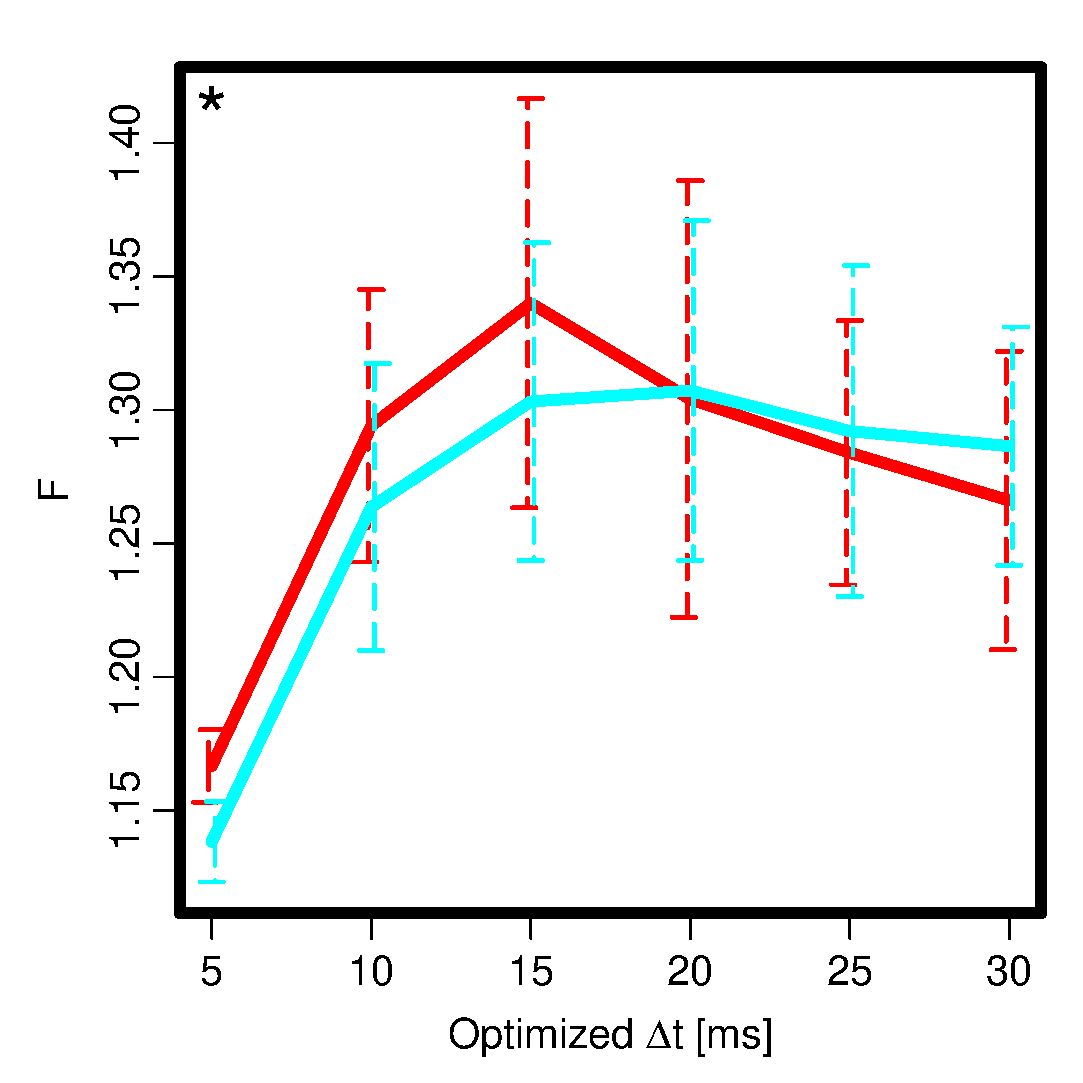
\includegraphics[width=0.8\columnwidth]{./Images_Result/Tsuishi_Rerative_F.eps} 
         \caption{F}
         \label{Tsuishi_Rerative_F}
       \end{subfigure}
       \begin{subfigure}{0.5\columnwidth}
         \centering
         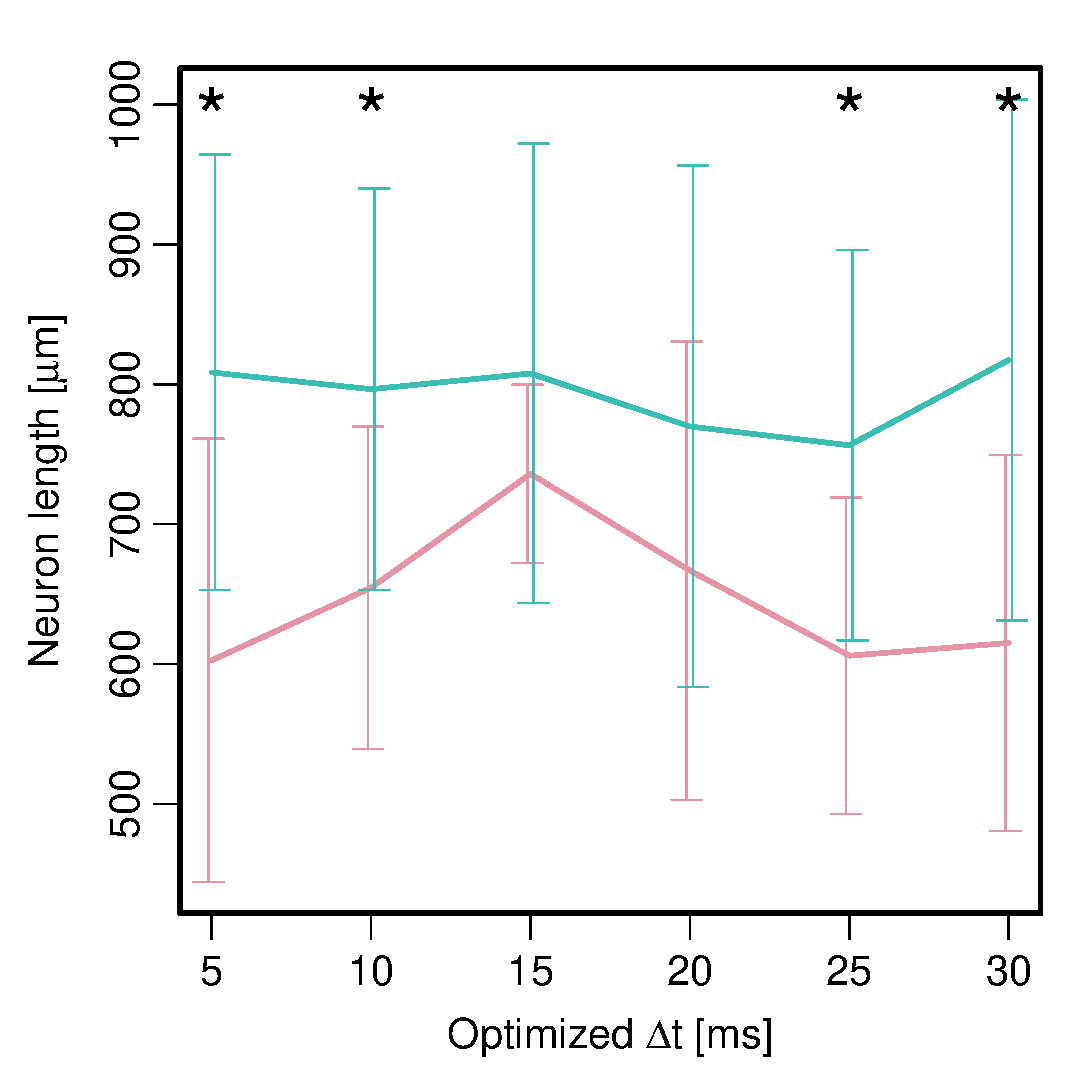
\includegraphics[width=0.8\columnwidth]{./Images_Result/Tsuishi_Rerative_TREE_length.eps} 
         \caption{$BD9$5(B}
         \label{Tsuishi_Rerative_length}
       \end{subfigure}

       \begin{subfigure}{0.5\columnwidth}
         \centering
         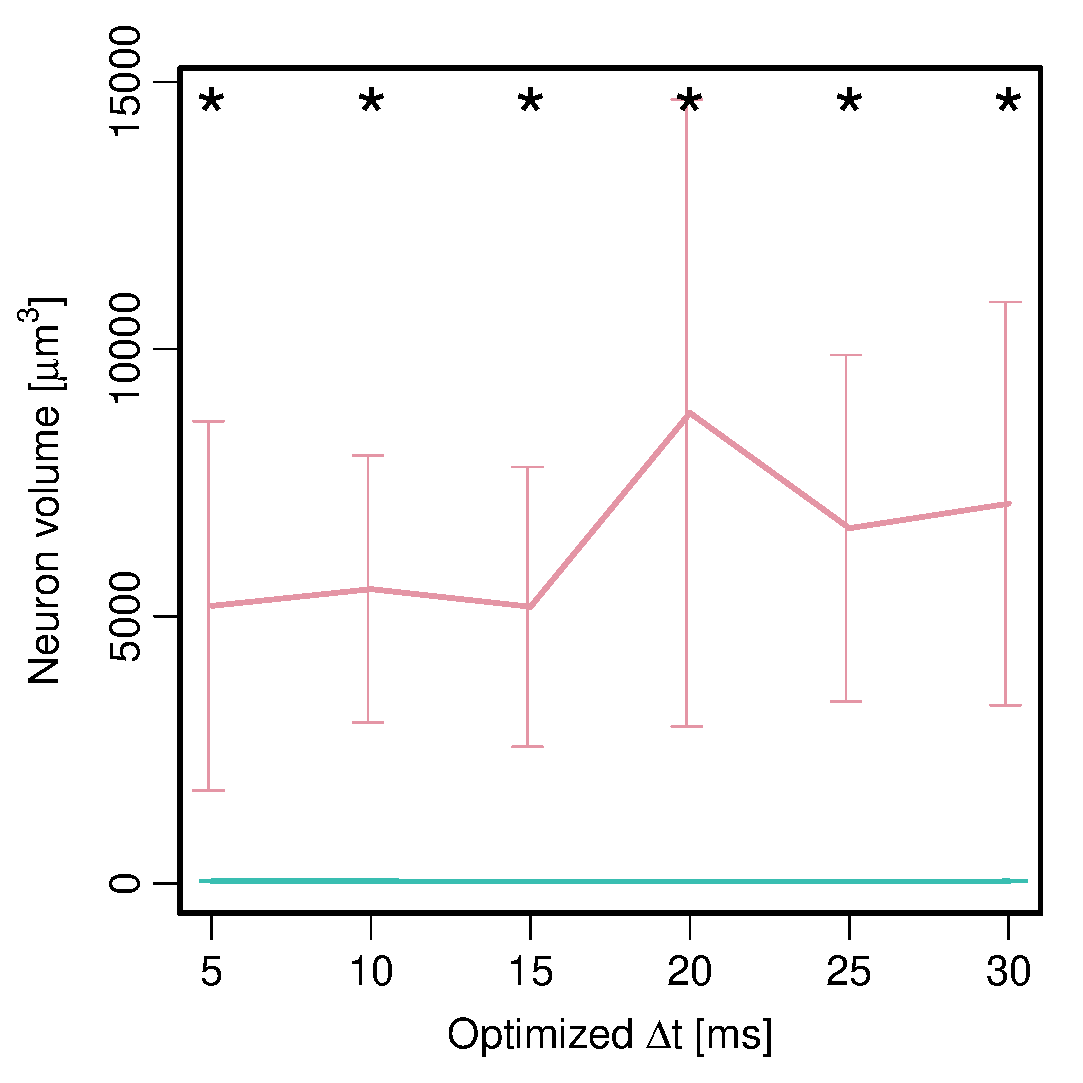
\includegraphics[width=0.8\columnwidth]{./Images_Result/Tsuishi_Rerative_TREE_volume.eps} 
         \caption{$BBN@Q(B}
         \label{Tsuishi_Rerative_volume}
       \end{subfigure}
       \begin{subfigure}{0.5\columnwidth}
         \centering
         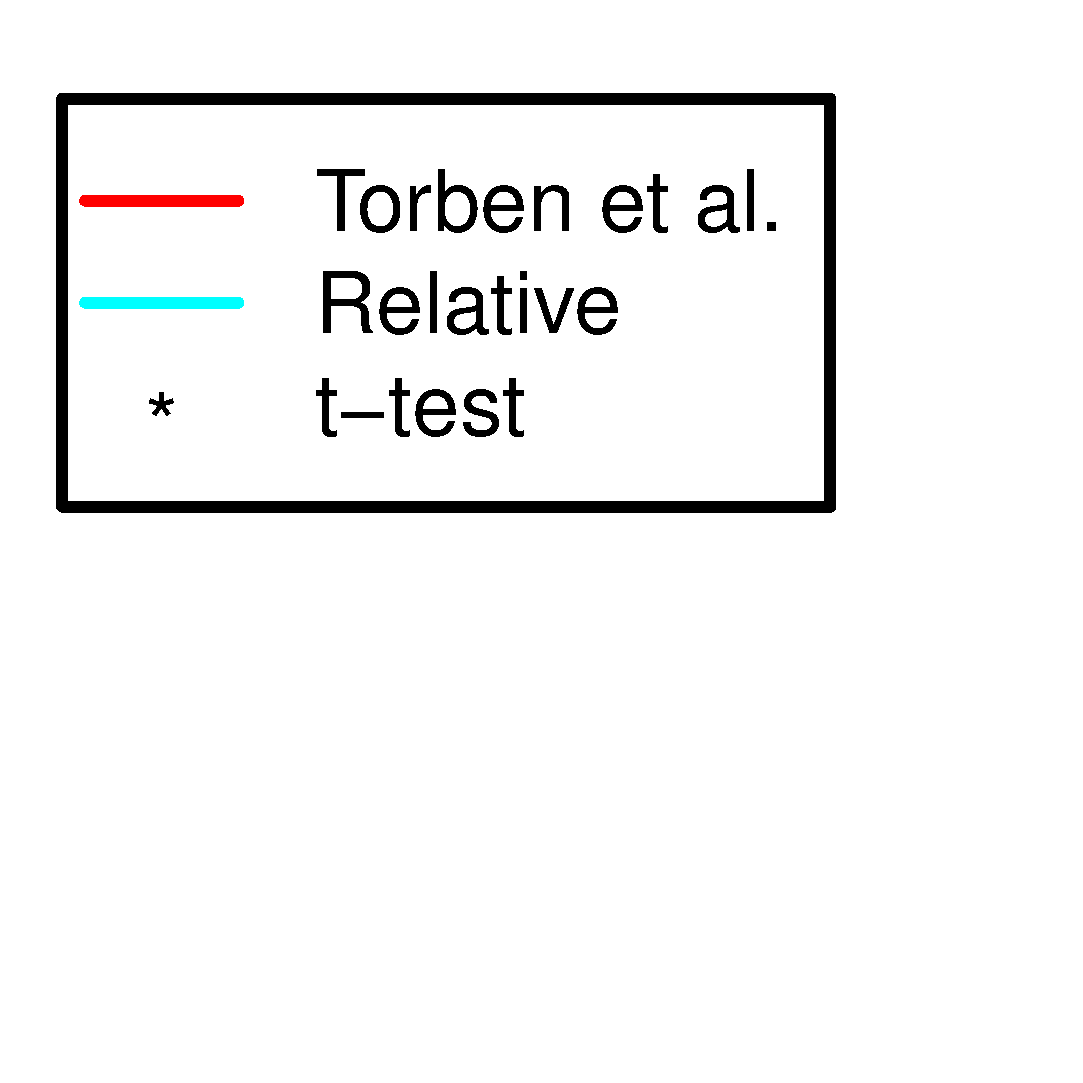
\includegraphics[width=0.8\columnwidth]{./Images_Result/Tsuishi_Rerative_legend.eps} 
       \end{subfigure}

       \caption{$B@h9T8&5f<jK!$H$NHf3S(B1}
       \label{Tsuishi_Rerative1}
     \end{figure}

     \begin{figure}[H]
       \begin{subfigure}{0.5\columnwidth}
         \centering
         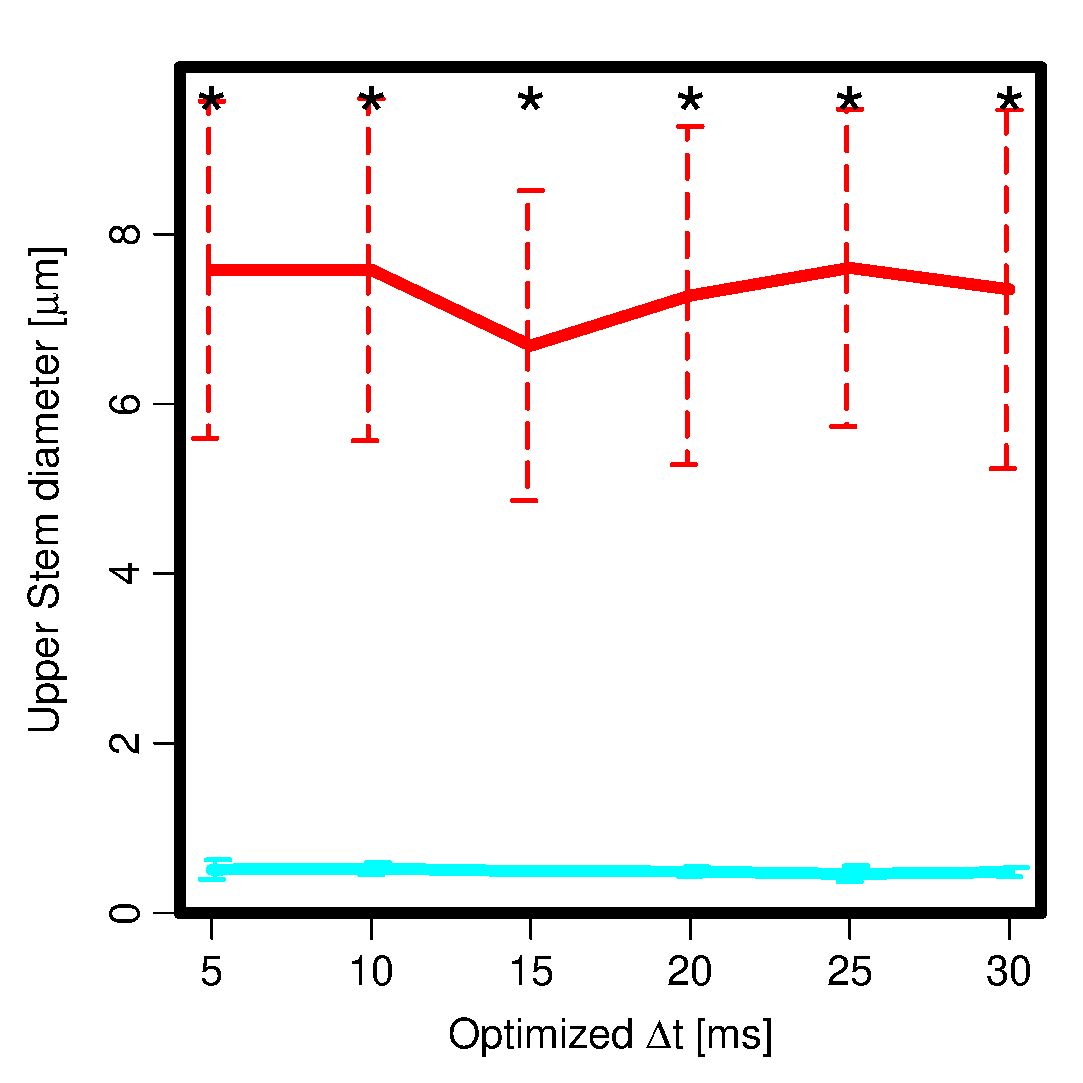
\includegraphics[width=0.8\columnwidth]{./Images_Result/Tsuishi_Rerative_Upper_Diam.eps} 
         \caption{Upper Dendrite$B$ND>7B(B}
         \label{Tsuishi_Rerative_Upper_Diam}
       \end{subfigure}
       \begin{subfigure}{0.5\columnwidth}
         \centering
         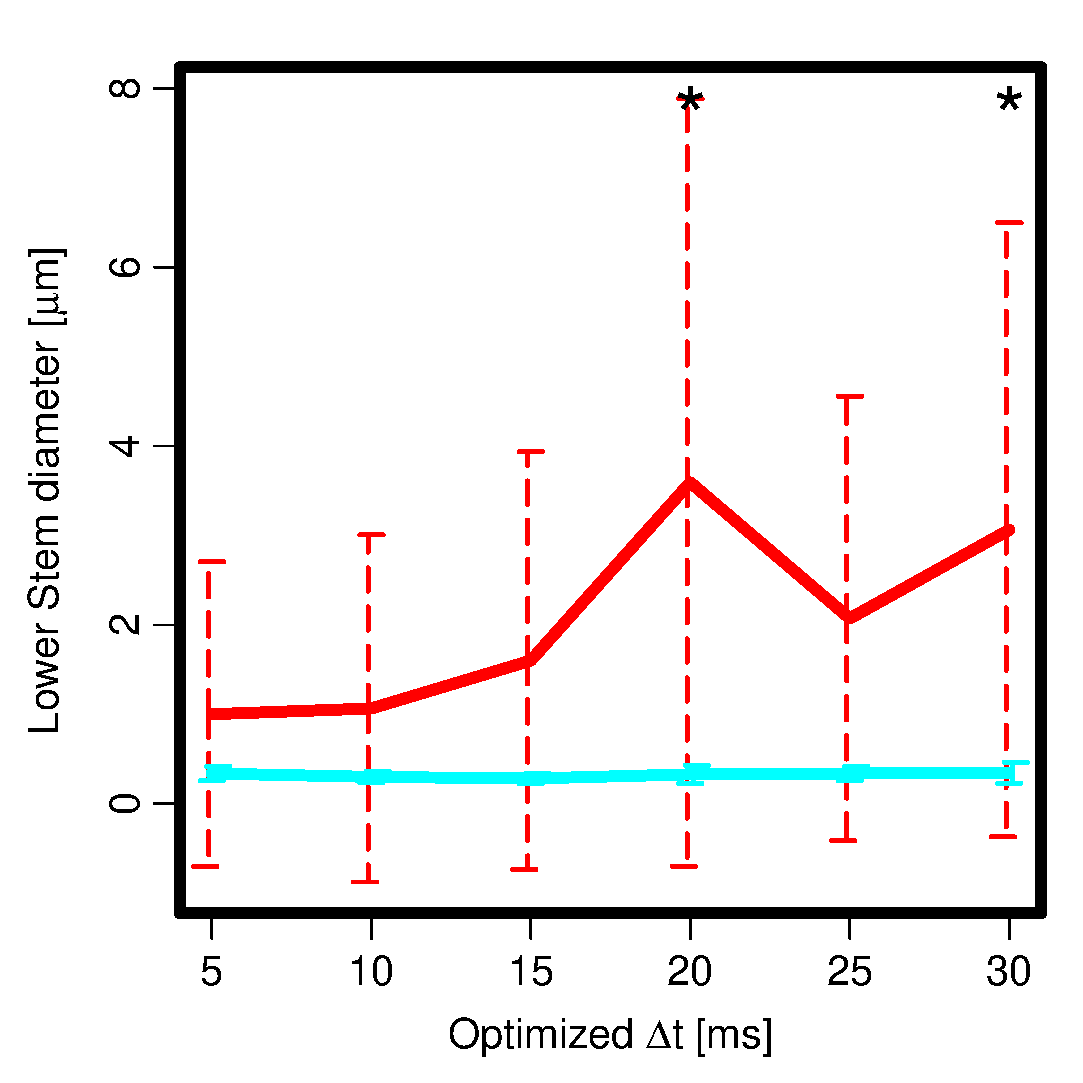
\includegraphics[width=0.8\columnwidth]{./Images_Result/Tsuishi_Rerative_Lower_Diam.eps} 
         \caption{Lower Dendrite$B$ND>7B(B}
         \label{Tsuishi_Rerative_Lower_Diam}
       \end{subfigure}
       %% \begin{subfigure}{0.3\columnwidth}
       %%   \centering
       %%   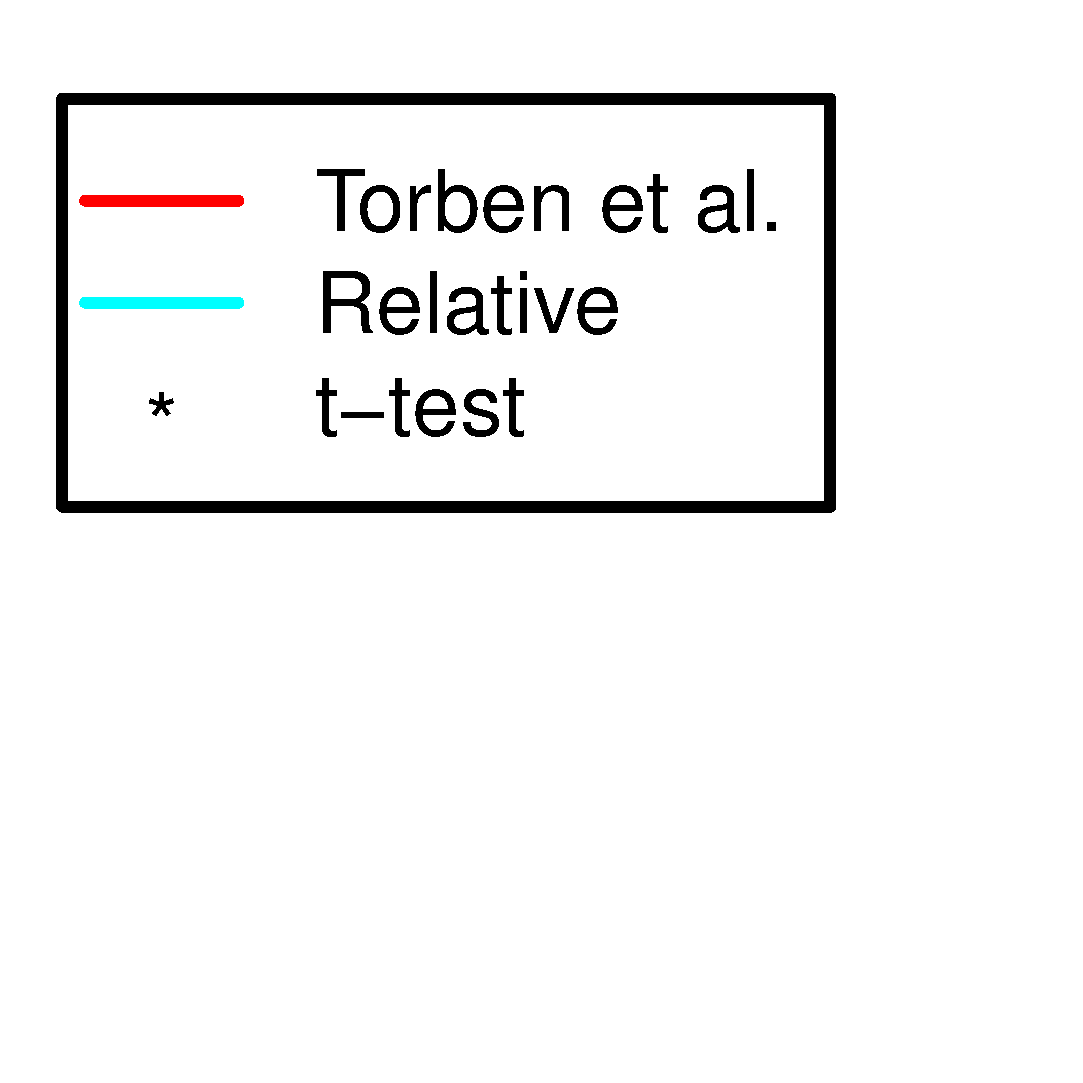
\includegraphics[width=\columnwidth]{./Images_Result/Tsuishi_Rerative_legend.eps} 
       %% \end{subfigure}
       \caption{$B@h9T8&5f<jK!$H$NHf3S(B2}
       \label{Tsuishi_Rerative2}
     \end{figure}

     $B3F(B${\Delta}t$$B$K$*$$$F?^Cf>eIt$N@10u(B(${\star}$)$B$O(B, $B%&%'%k%A$N(Bt$B8!Dj(B(${\alpha} = 0.05$)$B$rMQ$$$F(B 
     $B@h9T8&5f<jK!(B(Torben et al)$B$HK\8&5f<jK!(B(Rerative)$B$NJ?6QCM$rHf3S$7$?:]$K(B, $BM-0Y:9$,$_$i$l$?$3$H$r<($9(B. 
     $B?^(B\ref{Tsuishi_Rerative_F}$B$H?^(B\ref{Tsuishi_Rerative_volume}$B$+$i$o$+$k$h$&$K(B, 2$B$D$N<jK!$N4V$G5!G=@-(B$F$$B$K$O$"$^$j:9$O8+$i$l$J$$$,(B
     $BBN@Q$OL@$i$+$K>.$5$/$J$C$F$$$k(B. 
     $B$^$?(B, 2$B$D$N<jK!(B(${\Delta}t = 15$[ms])$B$G@8@.$5$l$??@7P:YK&$NNc$r?^(B\ref{passive_morphos}$B$K<($9(B. 
%
% $B7ABVNc$O$G$-$?$iJ#?t$N$;$?$$(B, $BGH7A$b$N$;$?$$(B
%
     \begin{figure}[H]
       \begin{subfigure}{0.5\columnwidth}
         \centering
         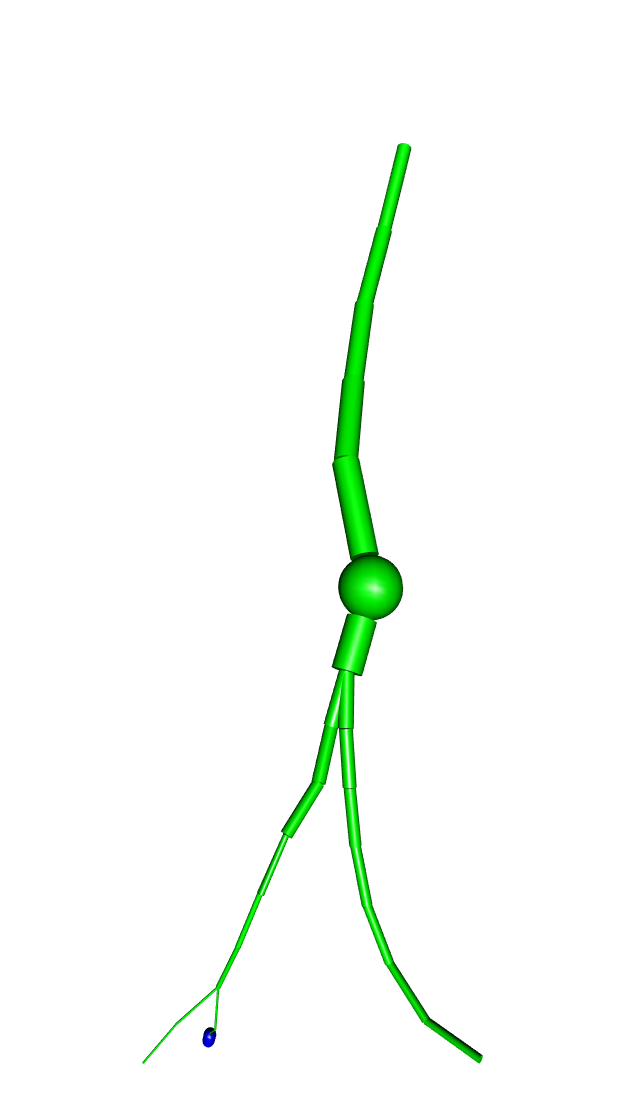
\includegraphics[width=0.7\columnwidth]{./Images_Result/alfa_sample.png} 
         \caption{$B@h9T8&5f<jK!(B}
         \label{Tsuishi_sampel}
       \end{subfigure}
       \begin{subfigure}{0.5\columnwidth}
         \centering
         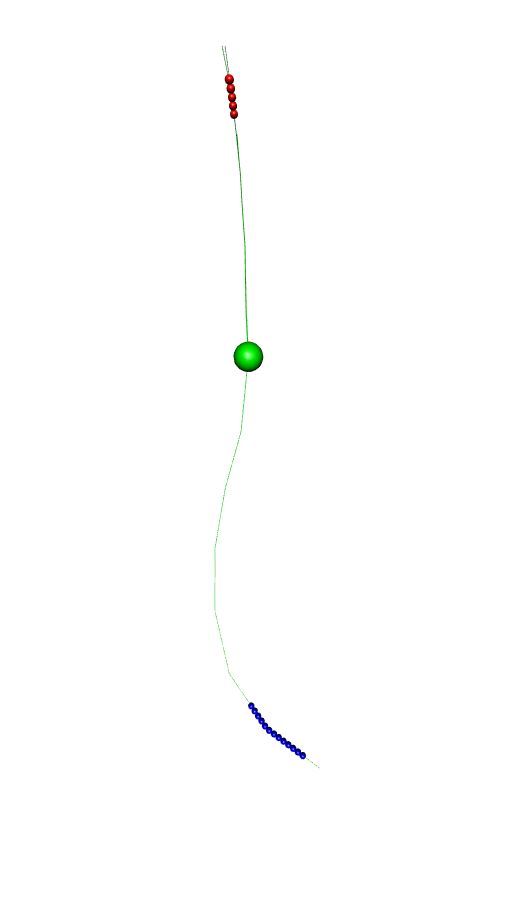
\includegraphics[width=0.5\columnwidth]{./Images_Result/rerative_sample.png}
         \caption{$BK\8&5f<jK!(B}
         \label{Rerative_sampel}
       \end{subfigure}
       \caption{Passive$B$J?@7P:YK&$N7ABVNc(B}
       \label{passive_morphos}
     \end{figure}

     %
     % $B%7%J%W%90LCV!"D9$5$N%0%i%U$O$b$&>/$72C9)$7$F$+$i=P$7$?J}$,$$$$(B
     %
     %

 \section{Ka$B%A%c%M%k$rMQ$$$?>l9g$N7k2L(B}
   $B?^(B\ref{Ka_Result1}, $B?^(B\ref{Ka_Result2}$B$K(BKa$B%A%c%M%k$rF3F~$7$?:]$N7k2L$r<($9(B. $B?^Cf$N(BGausian$B$O%3%s%@%/%?%s%9J,I[MM<0$K(B
   $B%,%&%9J,I[$rMQ$$$F$*$j(B, Liner$B$O@~7AJ,I[$rMQ$$$?>l9g$N7k2L$G$"$k(B.
   $B$^$?(B-reduced$B$O$=$l$>$l$N%3%s%@%/%?%s%9J,I[MM<0$G8DBNI>2A$K%3%s%@%/%?%s%9NL$X$N9MN8$rF3F~$7$?>l9g$N7k2L$G$"$k(B. \\
   $B%0%i%U>eIt$N5-9f$O3F(B${\Delta}t$$B$K$*$$$F(B, $B%&%'%k%A$N(Bt$B8!Dj(B($\alpha = 0.05$)$B$r9T$$M-0U:9$,$_$i$l$?$3$H$r(B
   $B<($7$F$$$k(B. $B5-9f(B($\star$)$B$OK\8&5f<jK!$N(BPassive$B$N7k2L$H(BGausian, Liner$B$N7k2L$rHf3S$7(B, $B$=$l$>$l$N?'$G<($7$F$$$k(B.
   $B5-9f(B($\#$)$B$O(BGausian$B$H(Breduced-Gausian, Liner$B$H(Breduced-Liner$B$NAH$GHf3S$r9T$C$?7k2L$G$"$k(B.
   $B$^$?5-9f(B($+$)$B$O(Breduced-Gausian$B$H(Breduced-Liner$B$rHf3S$7$?7k2L$G$"$k(B.
   \vspace{-0.5cm}
     \begin{figure}[H]
       \begin{subfigure}{0.5\columnwidth}
         \centering
         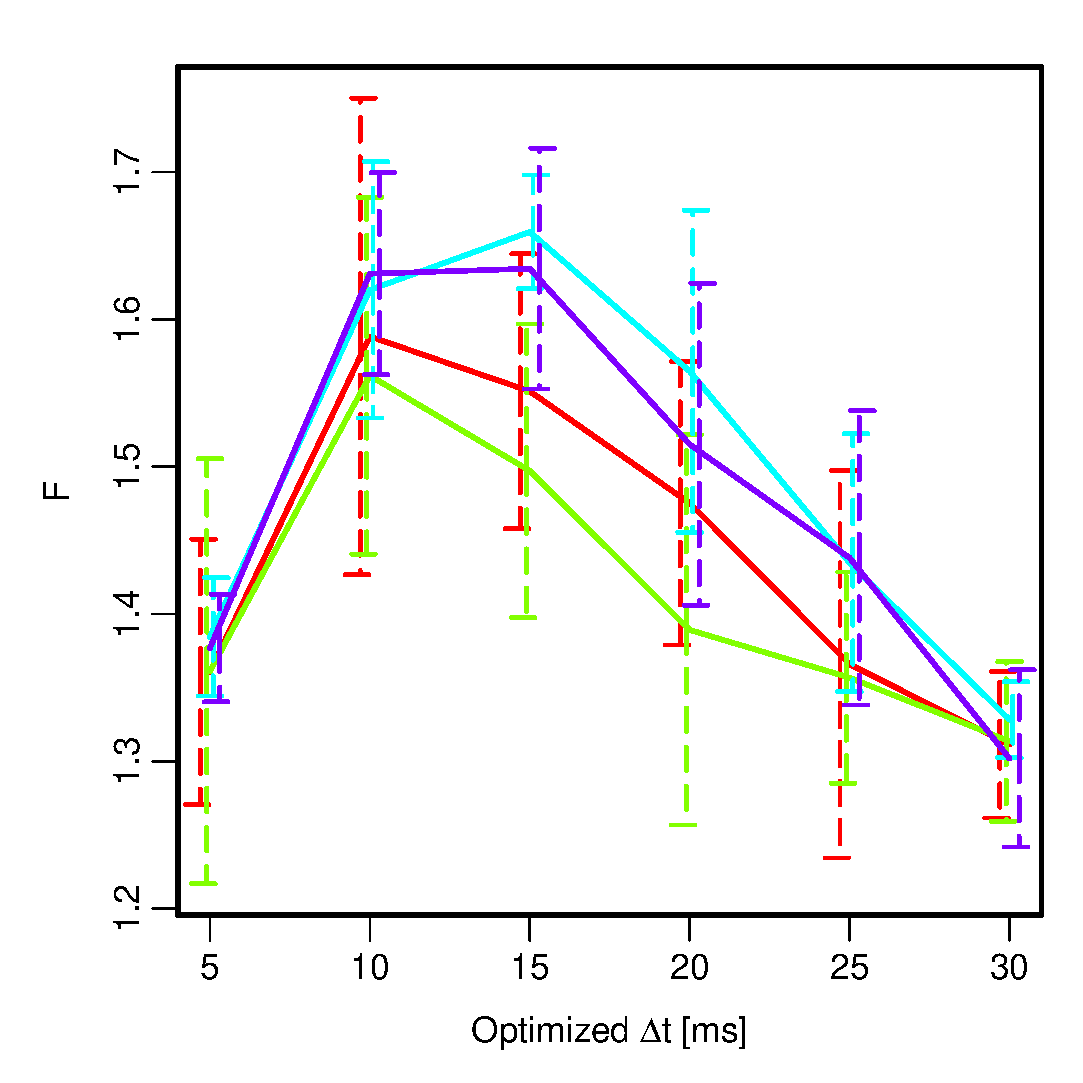
\includegraphics[width=0.8\columnwidth]{./Images_Result/k_test_F.eps}
         \caption{F}
         \label{k_F}
       \end{subfigure}
       \begin{subfigure}{0.5\columnwidth}
         \centering
         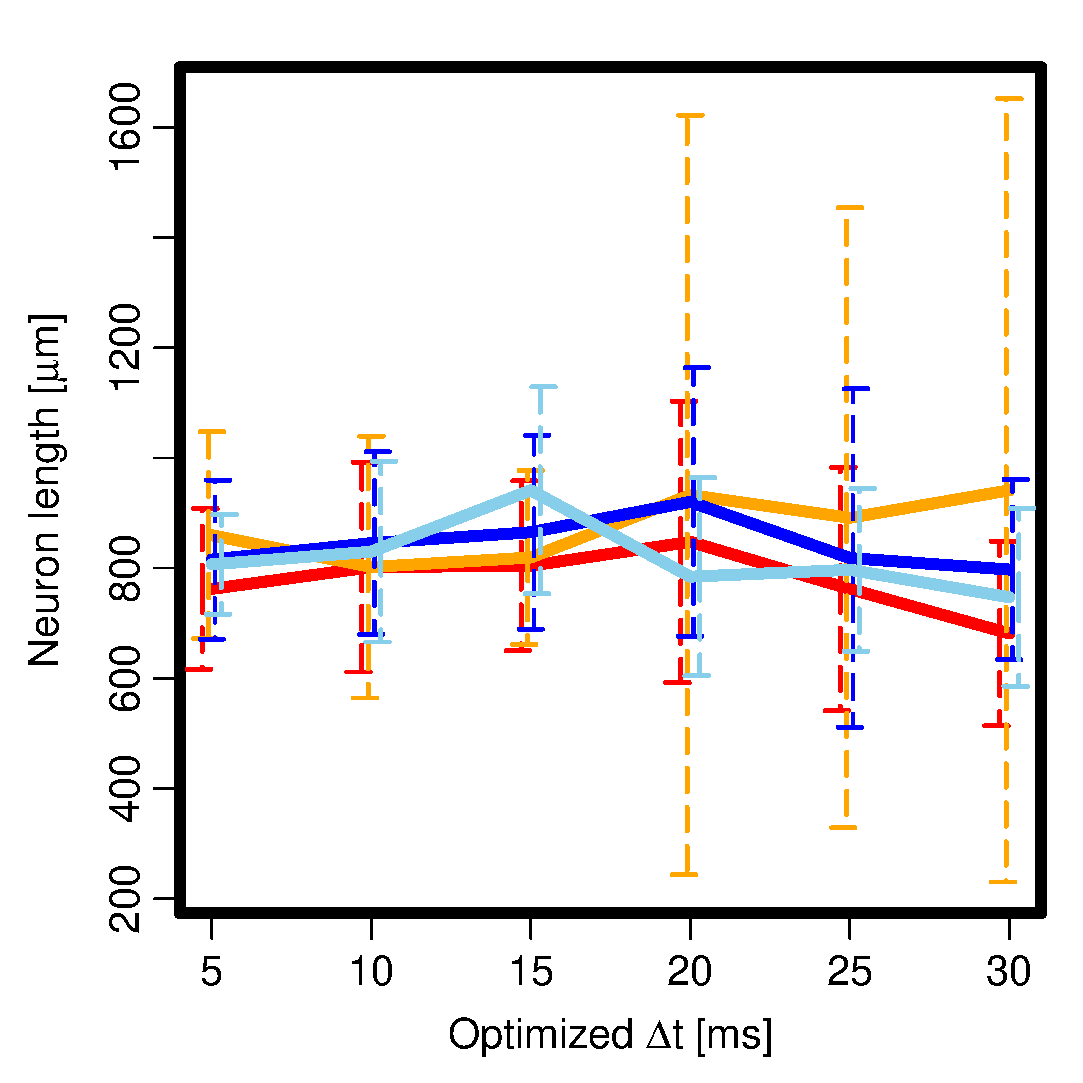
\includegraphics[width=0.8\columnwidth]{./Images_Result/k_test_TREE_length.eps} 
         \caption{$BD9$5(B}
         \label{k_TREE_length}
       \end{subfigure}

       \begin{subfigure}{0.5\columnwidth}
         \centering
         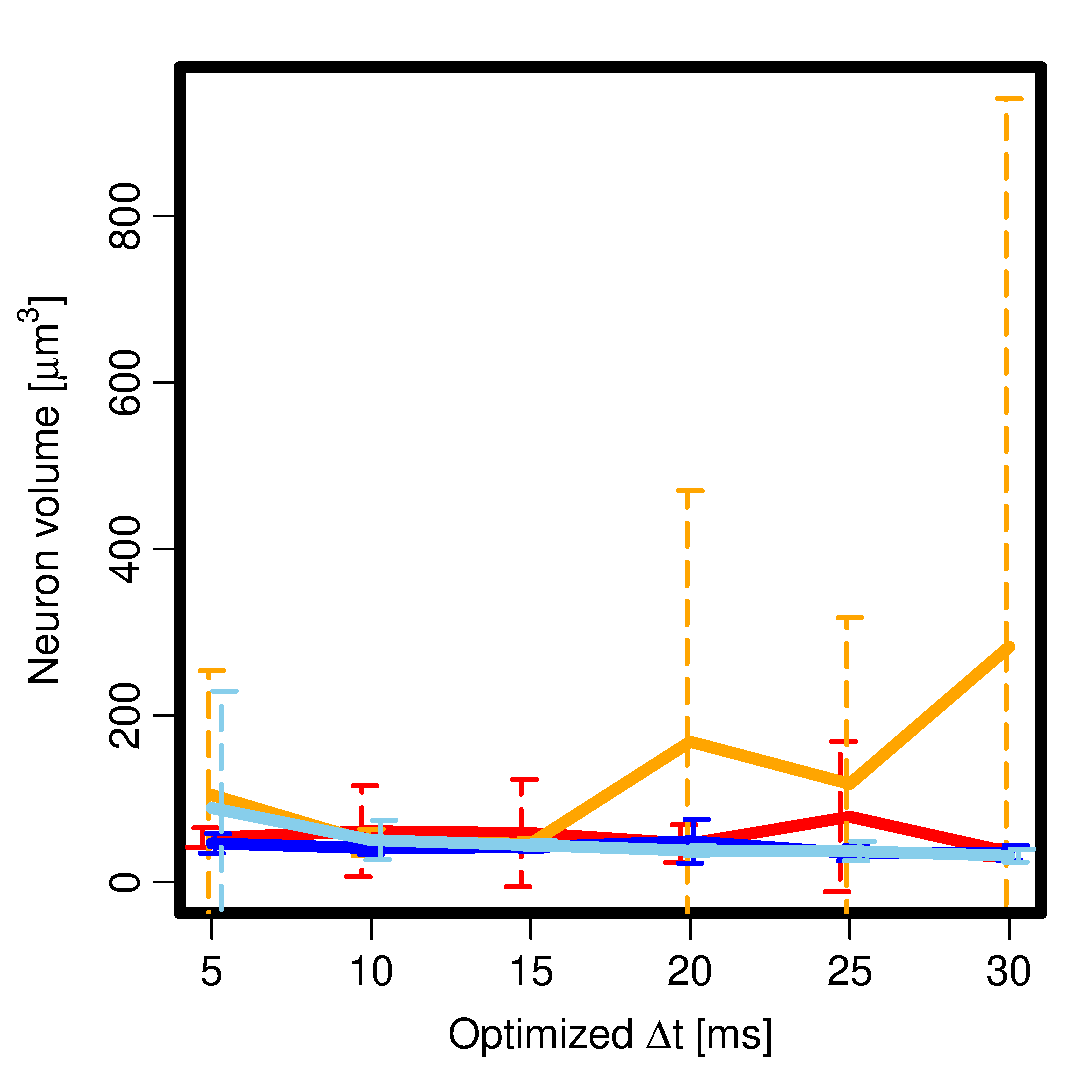
\includegraphics[width=0.8\columnwidth]{./Images_Result/k_test_TREE_volume.eps}
         \caption{$BBN@Q(B}
         \label{k_TREE_volume}
       \end{subfigure}
       \begin{subfigure}{0.5\columnwidth}
         \centering
         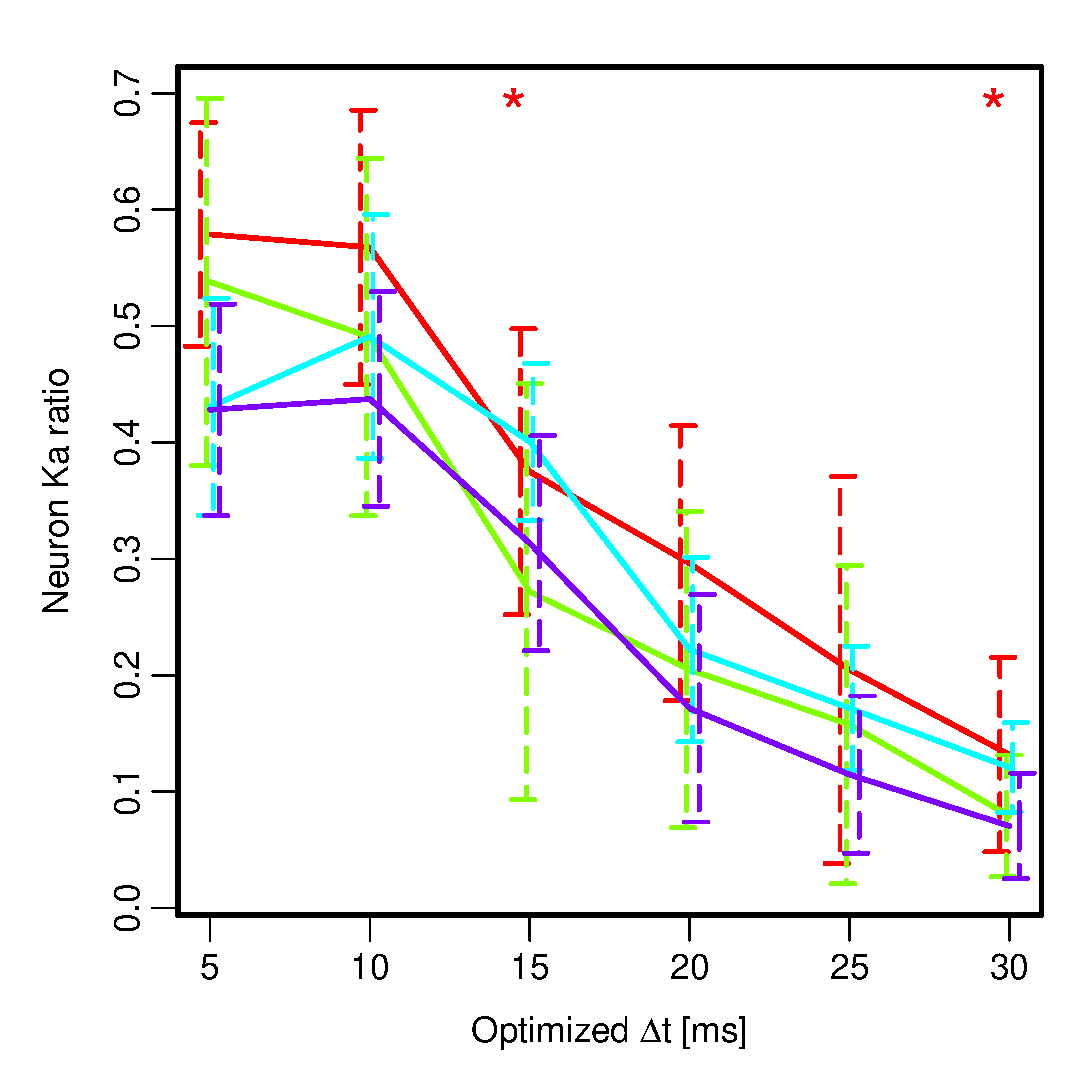
\includegraphics[width=0.8\columnwidth]{./Images_Result/k_test_TREE_K_ratio.eps}
         \caption{Ka$B%3%s%@%/%?%s%94^M-N((B}
         \label{k_TREE_K_ratio}
       \end{subfigure}

       \vspace{-0.3cm}
       \begin{subfigure}{0.5\columnwidth}
         \centering
         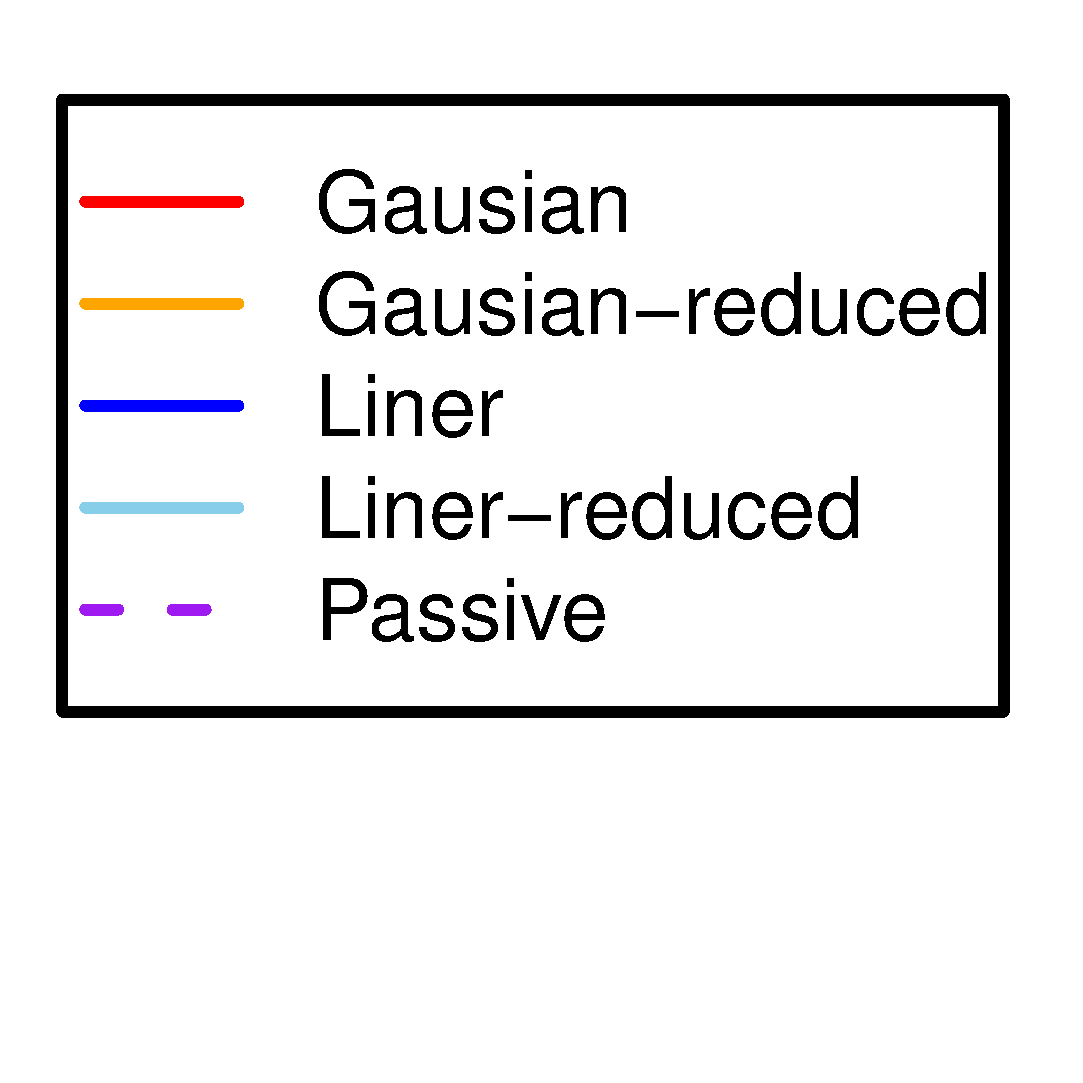
\includegraphics[width=0.6\columnwidth]{./Images_Result/k_test_legend.eps} 
       \end{subfigure}
       \begin{subfigure}{0.5\columnwidth}
         \centering
         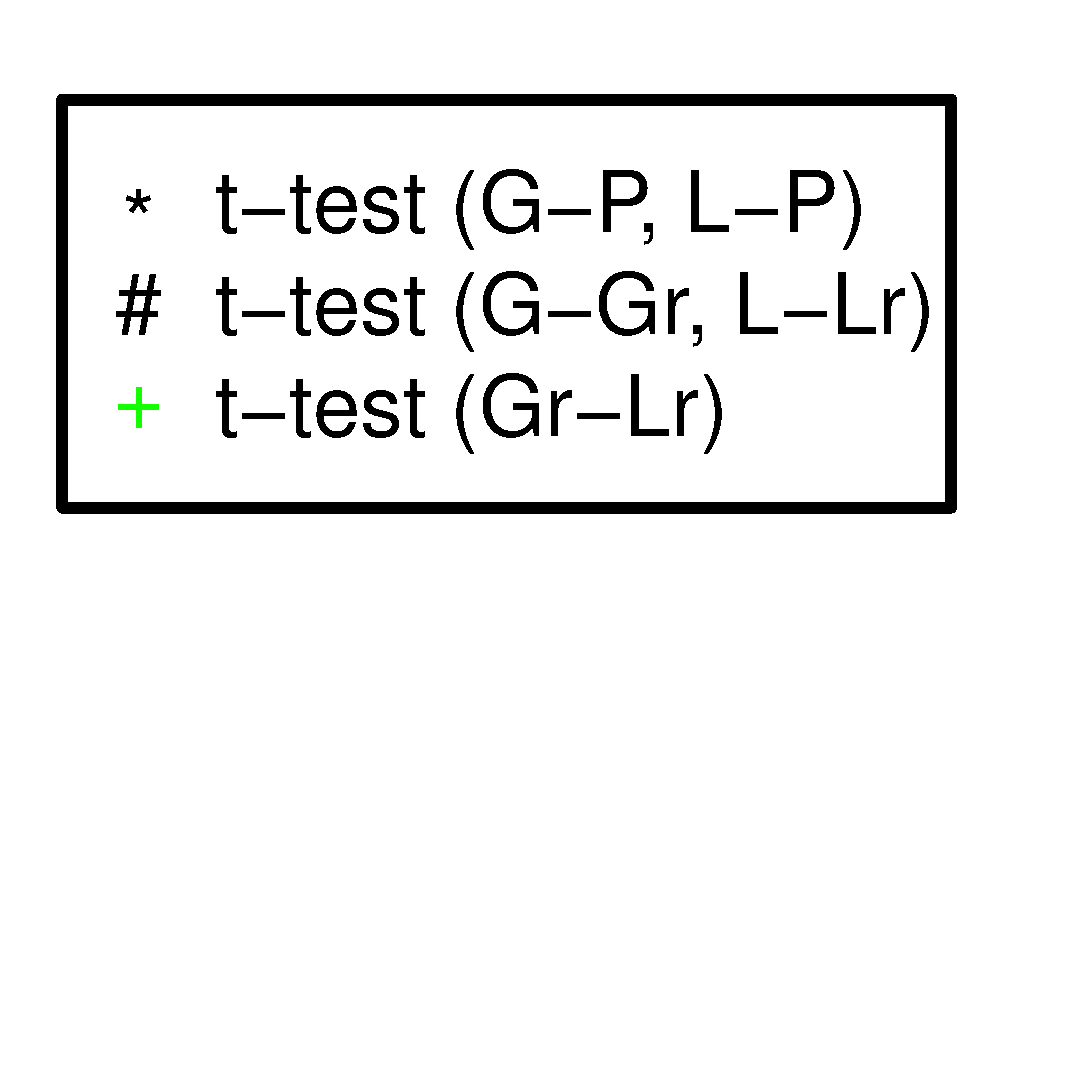
\includegraphics[width=0.6\columnwidth]{./Images_Result/test_legend.eps} 
       \end{subfigure}

       \vspace{-1.6cm}
       \caption{Ka$B%A%c%M%k$rF3F~$7$?:]$N7k2L(B1} %$B%Z!<%8%l%$%"%&%H$,7hDj$7$F$+$iHyD4@0$9$k(B
       \label{Ka_Result1}
     \end{figure}

     \begin{figure}[H]
       \begin{subfigure}{0.5\columnwidth}
         \centering
         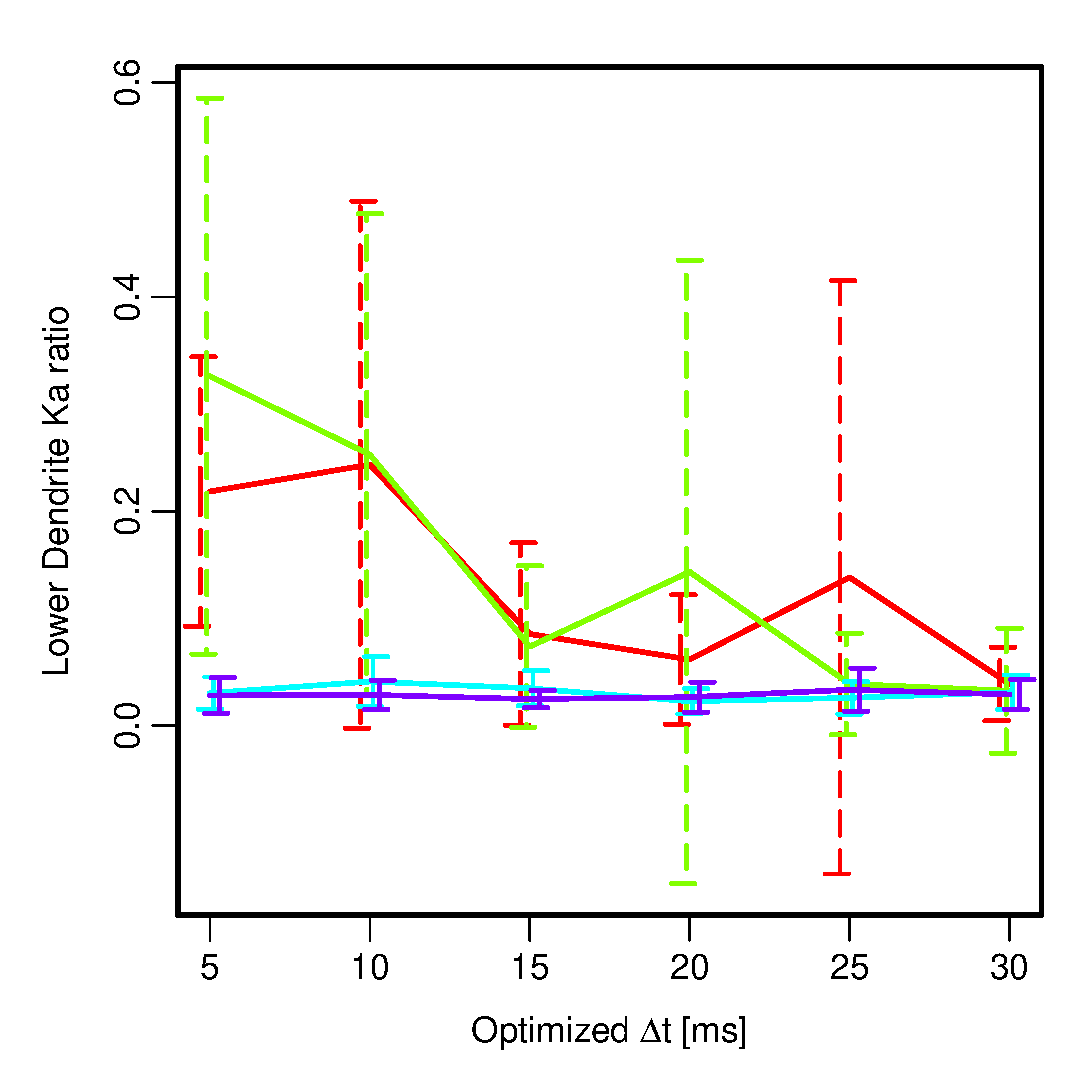
\includegraphics[width=0.8\columnwidth]{./Images_Result/k_test_Lower_K_ratio.eps}
         \caption{Lower Dendrite$B$N(BKa$B%3%s%@%/%?%s%94^M-N((B}
         \label{k_lower_ratio}
       \end{subfigure}
       \begin{subfigure}{0.5\columnwidth}
         \centering
         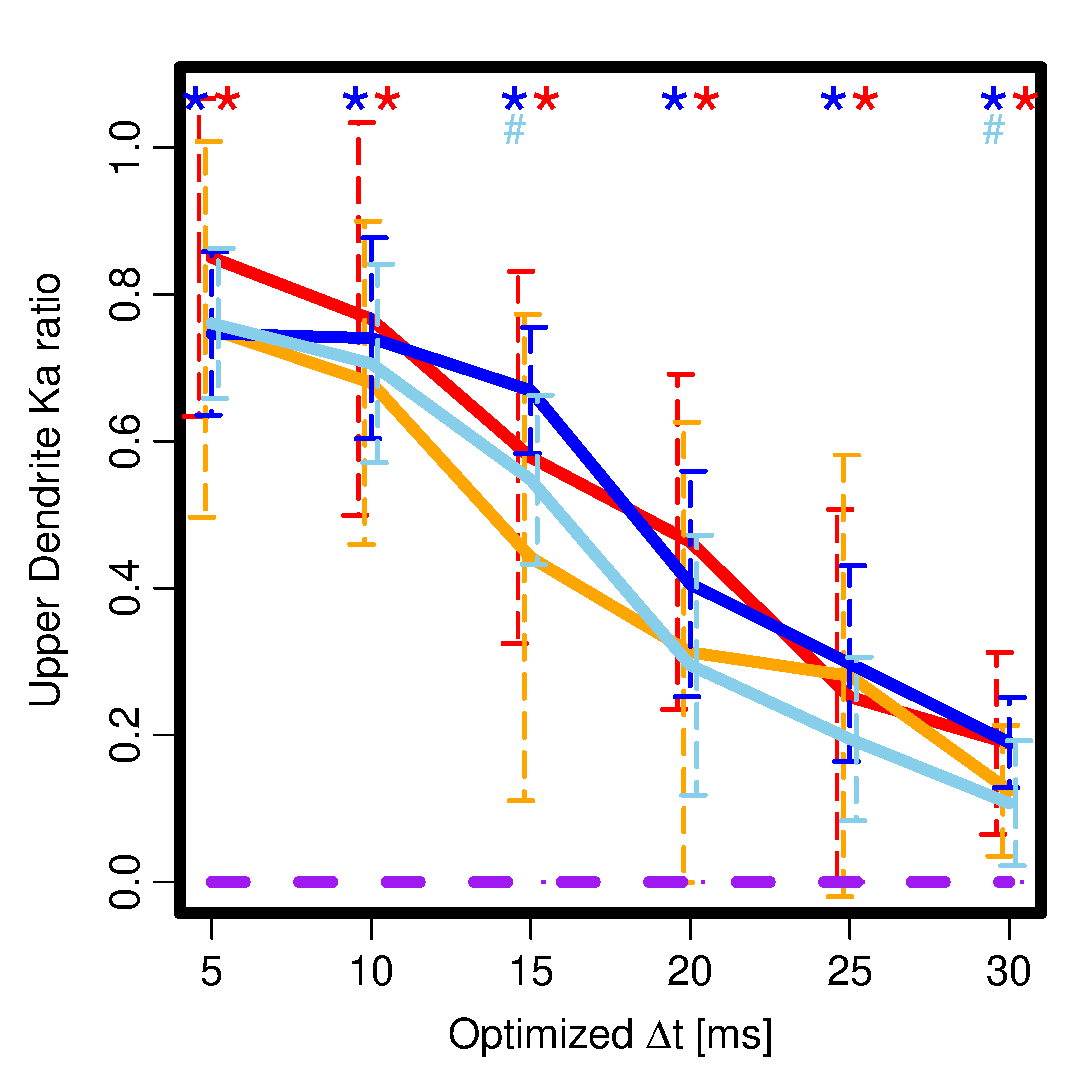
\includegraphics[width=0.8\columnwidth]{./Images_Result/k_test_Upper_K_ratio.eps}
         \caption{Upper Dendrite$B$N(BKa$B%3%s%@%/%?%s%94^M-N((B}
         \label{k_upper_ratio}
       \end{subfigure}

       \vspace{-0.3cm}
       \begin{subfigure}{0.5\columnwidth}
         \centering
         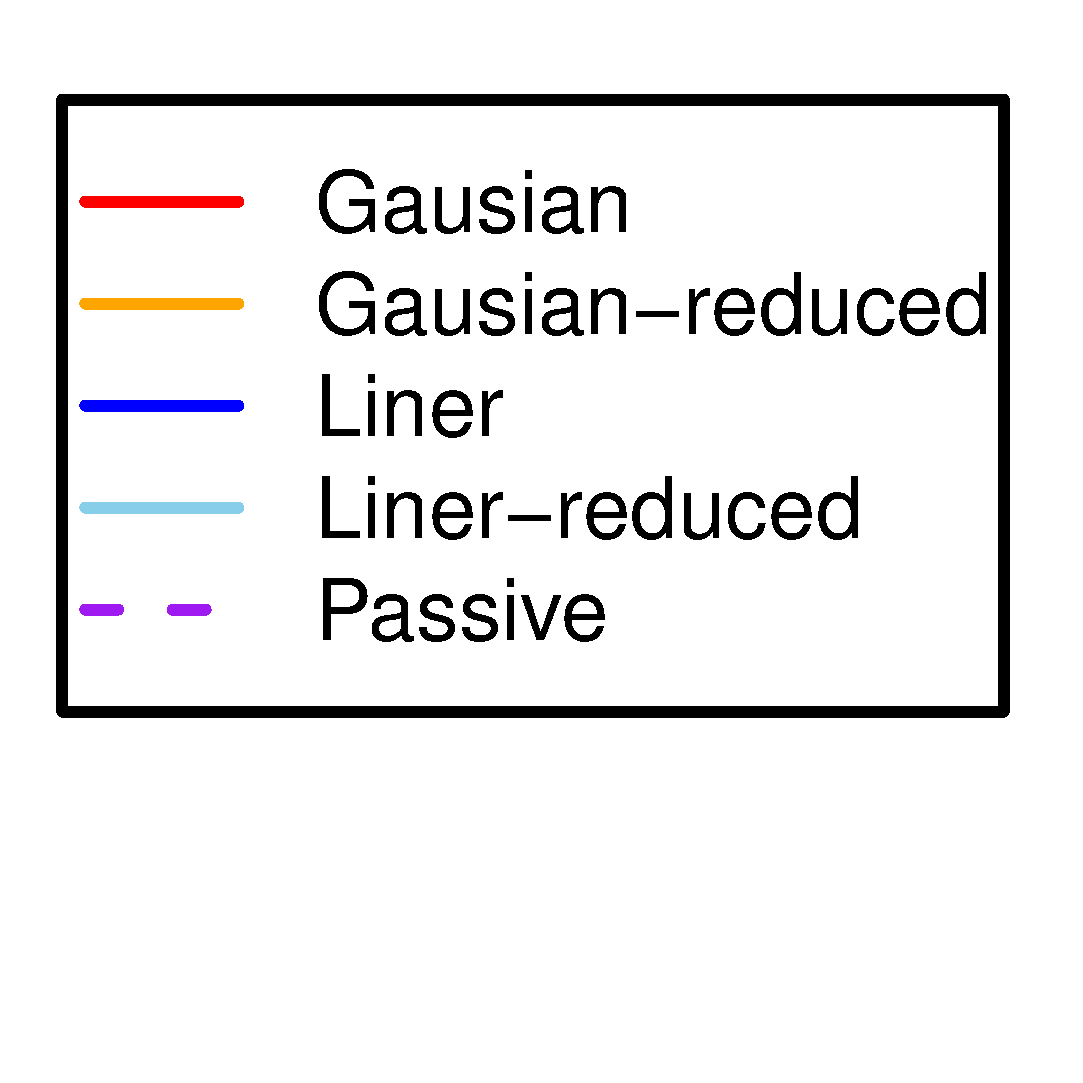
\includegraphics[width=0.6\columnwidth]{./Images_Result/k_test_legend.eps} 
       \end{subfigure}
       \begin{subfigure}{0.5\columnwidth}
         \centering
         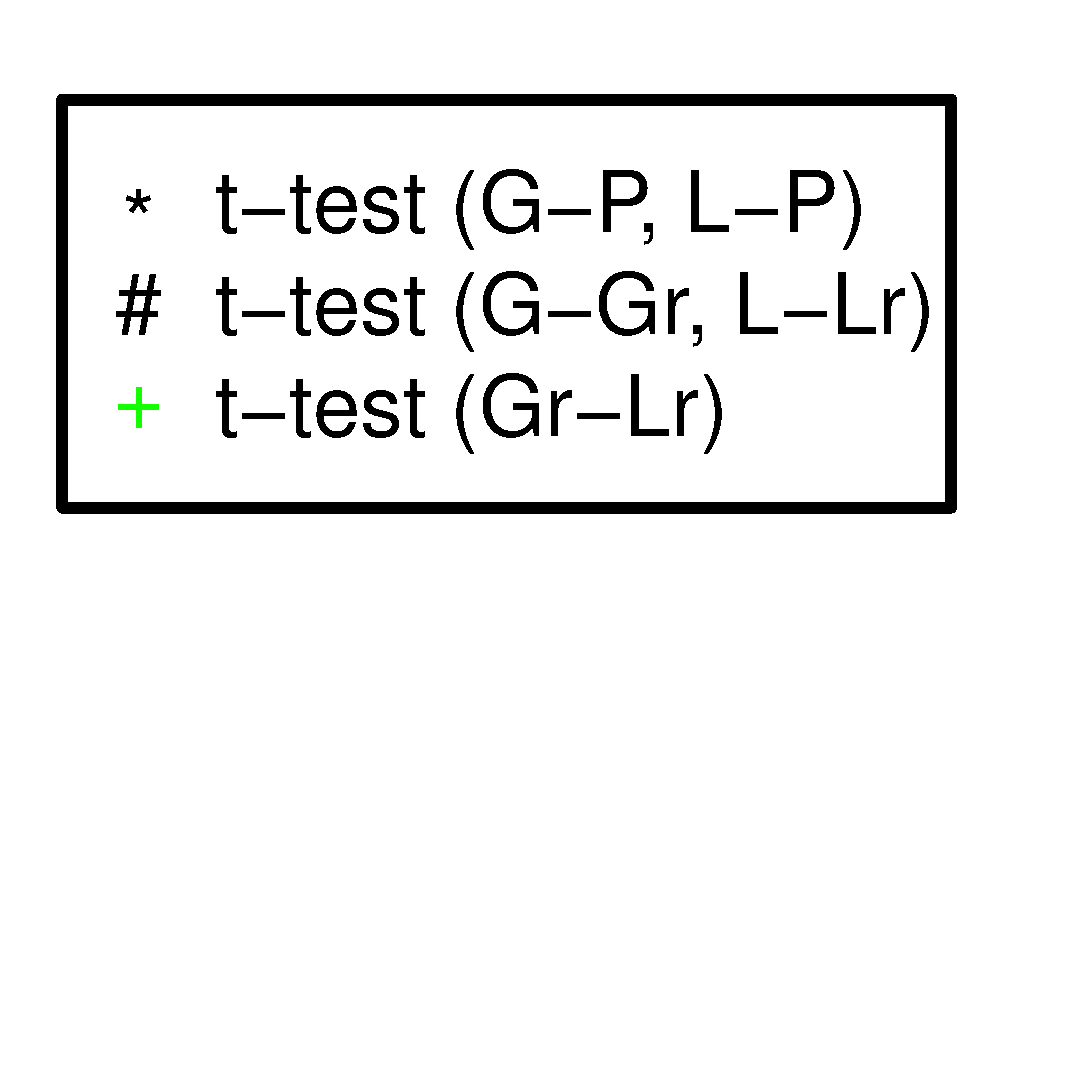
\includegraphics[width=0.6\columnwidth]{./Images_Result/test_legend.eps} 
       \end{subfigure}

       \vspace{-1.6cm}
       \caption{Ka$B%A%c%M%k$rF3F~$7$?:]$N7k2L(B2} %$B%Z!<%8%l%$%"%&%H$,7hDj$7$F$+$iHyD4@0$9$k(B
       \label{Ka_Result2}
     \end{figure}

  $B?^(B\ref{k_F}$B$h$j(BKa$B%3%s%@%/%?%s%9$rF3F~$7$?$3$H$G(BPassive$B$N>l9g$h$j$b(B$F$$BCM$,A}2C$7$F$$$k(B
  $B$3$H$,$o$+$k(B. $B@h9T8&5f$G$O(B${\Delta}t=5$[ms]$B$N$H$-$K:G$b9b$$(B$F$$BCM$,F@$i$l$F$$$?$,(B,
  $B$=$l$H$O0[$J$k7k2L$H$J$C$?(B. 
  $B?^(B\ref{k_TREE_K_ratio}$B$h$j%3%s%@%/%?%s%9$r9MN8$9$k>l9g$G$b?@7P:YK&(B
  $B$N(BKa$B%3%s%@%/%?%s%94^M-N($O$"$^$jJQ2=$,$J$$$3$H$,$o$+$k(B. \\
  $B?^(B\ref{k_morphos}$B$K:n@.$7$??@7P:YK&$N7ABVNc$r<($9(B. %$B$"$H$GD%$jD>$9(B
     
  \begin{figure}[H]
    \begin{subfigure}{0.5\columnwidth}
      \centering
      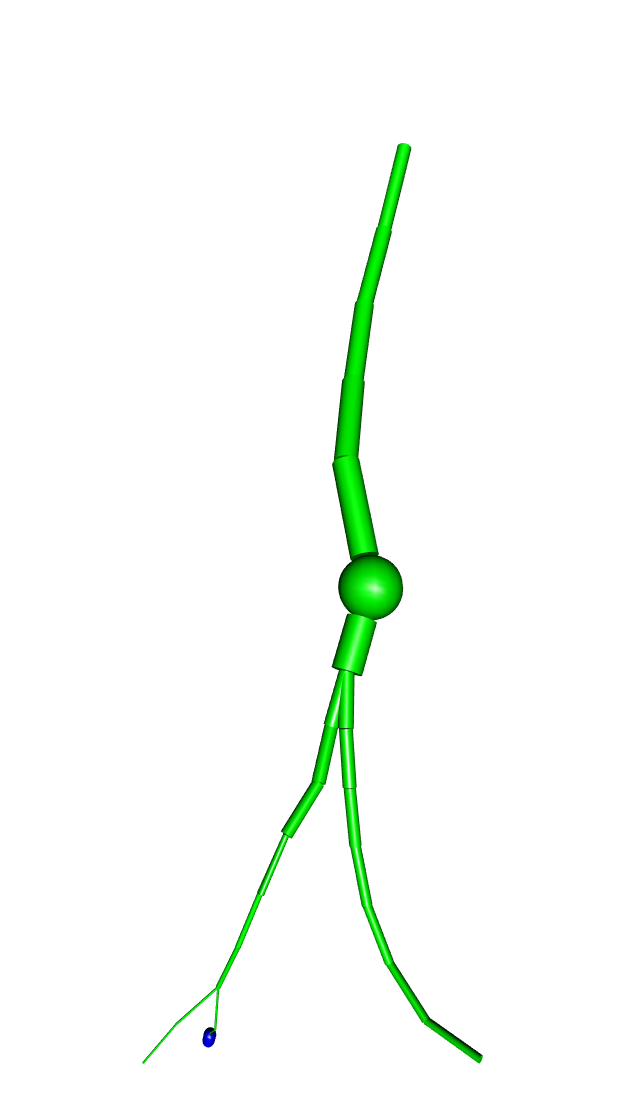
\includegraphics[width=0.5\columnwidth]{./Images_Result/alfa_sample.png} 
      \caption{$B@h9T8&5f<jK!(B}
      \label{Tsuishi_sampel}
    \end{subfigure}
    \begin{subfigure}{0.5\columnwidth}
      \centering
      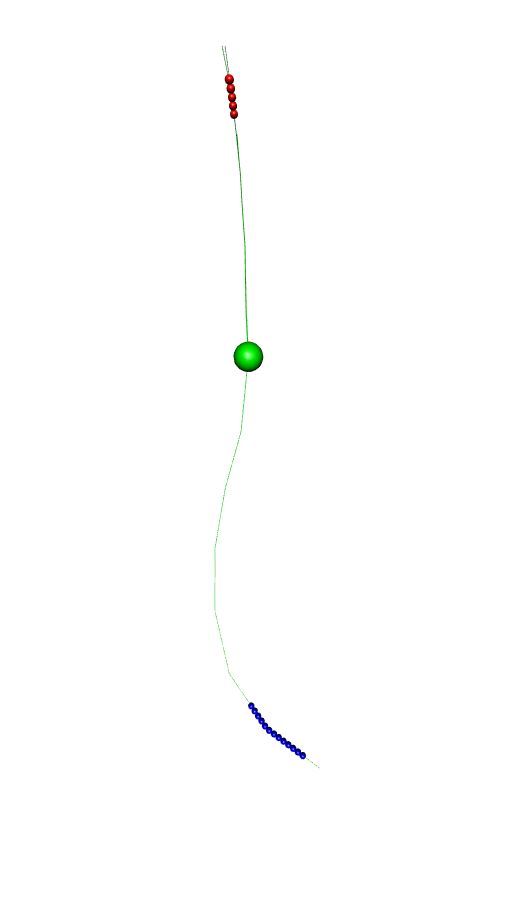
\includegraphics[width=0.3\columnwidth]{./Images_Result/rerative_sample.png}
      \caption{$BK\8&5f<jK!(B}
      \label{Rerative_sampel}
    \end{subfigure}
    \caption{Ka$B%3%s%@%/%?%s%9$rF3F~$7$??@7P:YK&$N7ABVNc(B}
    \label{k_morphos}
  \end{figure}

   $B$^$?(B, $B?^(B\ref{k_Ka_dist}$B$K(B${\Delta}t = 5$[ms]$B$N$H$-:n@.$7$??@7P:YK&$N(B
   $B%3%s%@%/%?%s%9J,I[$r<($9(B.
   $B?^(B\ref{k_liner_reduced_dist}$B$O@~7AJ,I[$rMQ$$(B, $B?^(B\ref{k_gaus_reduced_dist}
   $B$O%,%&%9J,I[$rMQ$$$F$$$k(B. $B$I$A$i$bI>2A<0$K$*$$$F%3%s%@%/%?%s%9NL$X$N9MN8$,$"$k>l9g(B
   $B$G$"$k(B. %$B%3%s%@%/%?%s%9$X$N9MN8$C$F$$$A$$$A8@$&$N$OLLE]$/$5$$(B
   $B?^$N2#<4$O<y>uFM5/>e$N0LCV$r;X<($7(B, $B?^Cf$N4]0u$O%7%J%W%9$N$D$$$F$$$k0LCV$r(B
   $BI=$7$F$$$k(B. $B?^Cf$G$O4]0u$,=E$J$j@~$N$h$&$K$J$C$F$$$k$,(B, $B$3$l$O%7%J%W%9$,8_$$$K(B
   $B6a$$0LCV$KJ,I[$7$F$$$k$?$a(B, 
          %
          %$B!!?^$r:n$jD>$9(B
          %
   \begin{figure}[H]
     \hspace*{-4cm}
     \begin{subfigure}{0.68\columnwidth}
       \centering
       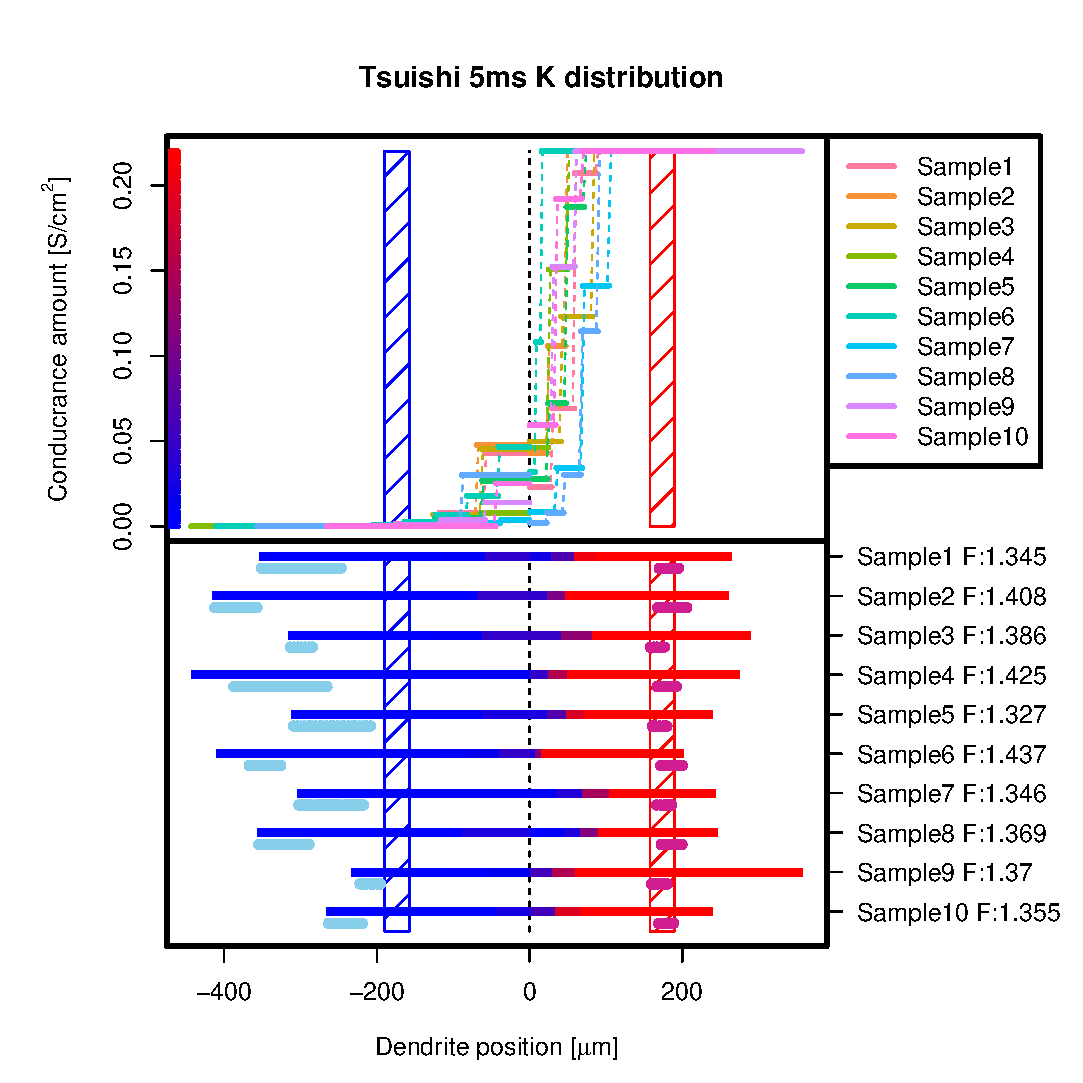
\includegraphics[width=\columnwidth]{./Images_Result/k_Rerative_liner_75_5_K_distribution_dt5.eps}
       \caption{$B@~7AJ,I[(B(reduced)}
       \label{k_liner_reduced_dist}
     \end{subfigure}
     \begin{subfigure}{0.68\columnwidth}
       \centering
       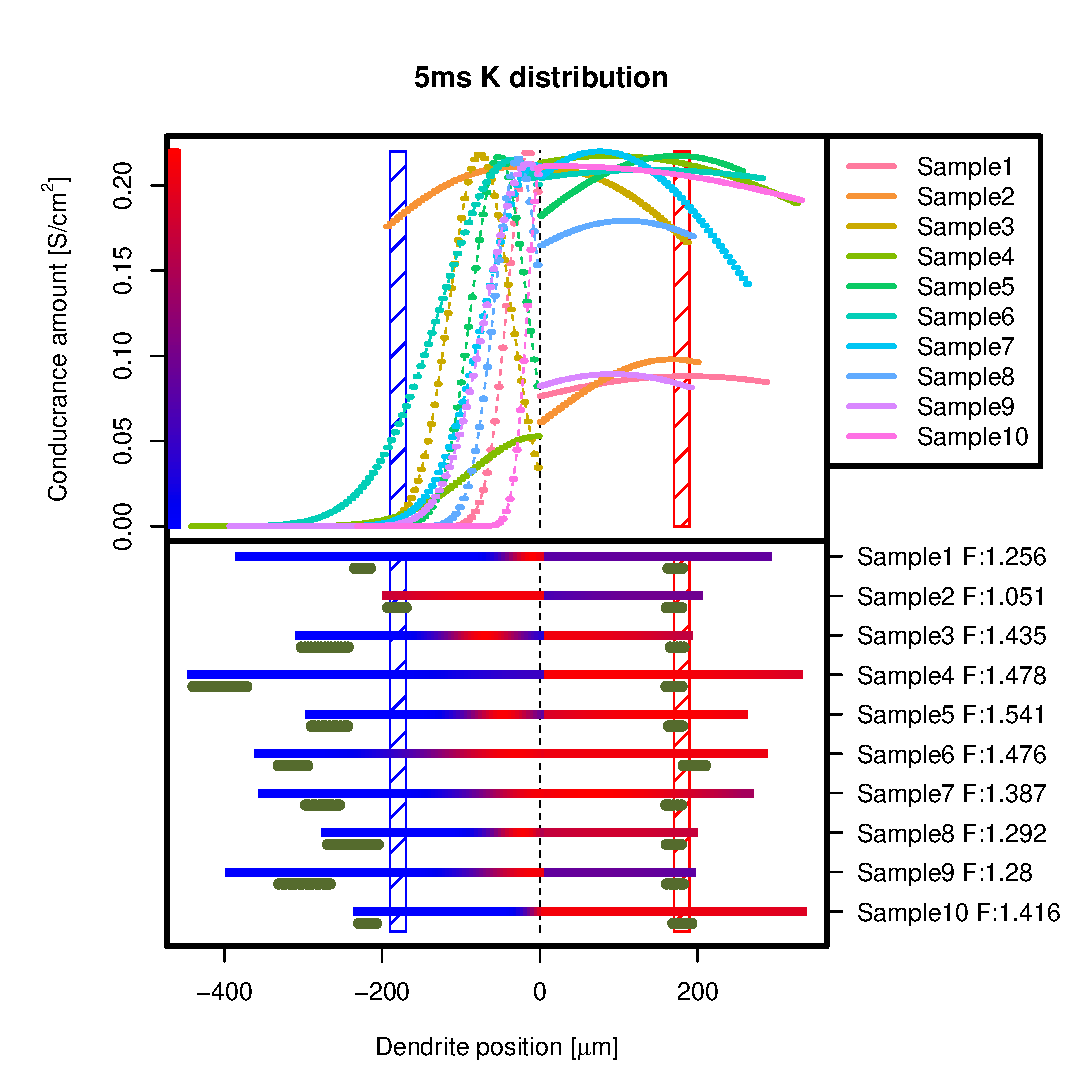
\includegraphics[width=\columnwidth]{./Images_Result/k_Rerative_Gaus_75_5_K_distribution_dt5.eps}
       \caption{$B%,%&%9J,I[(B(reduced)} %$B$3$N%,%&%9J,I[$N?^$O%7%J%W%F%#%C%/%>!<%s$r:n$jD>$7$?$[$&$,$$$$(B
       \label{k_gaus_reduced_dist}
     \end{subfigure}
     
     \begin{subfigure}{\columnwidth}
       \centering
       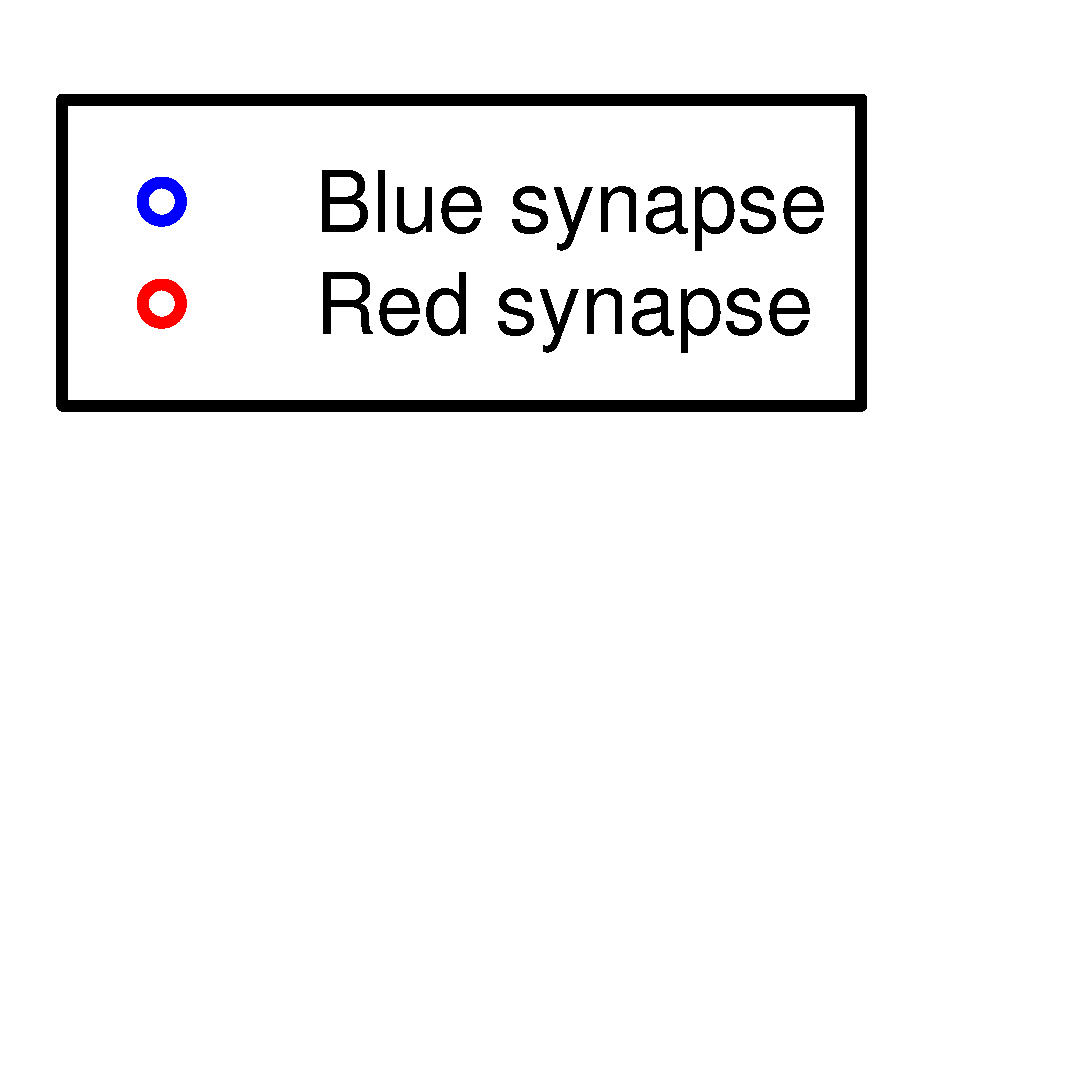
\includegraphics[width=0.35\columnwidth]{./Images_Result/Synapse_legend.eps} 
     \end{subfigure}
            
     \vspace{-3cm}
     \caption{${\Delta}t = 5$[ms], $B$G$N(BKa$B%3%s%@%/%?%s%9J,I[(B}
     \label{k_Ka_dist}
   \end{figure}

   $B?^(B\ref{k_gaus_reduced_dist}, $B?^(B\ref{k_upper_ratio}$B$+$i$o$+$k$h$&$K%,%&%9J,I[$rMQ$$$?>l9g(B
   $B$G$O(BUpper Dendrite$B$N:,85IU6a$G9b$$(BKa$B%3%s%@%/%?%s%9$NJ,I[$,8+$i$l$k(B.
   
 \section{CaT$B%A%c%M%k$rMQ$$$?>l9g$N7k2L(B}
   $B?^(B\ref{ca_result}$B$K(BCaT$B%A%c%M%k$rF3F~$7$?:]$N7k2L$r<($9(B.
   $BK^Nc$d8!Dj<jK!$H$=$N7k2L$N<($7J}$O?^(B\ref{Ka_Result1}$B$HF1MM$G$"$k(B.
    \vspace{-0.5cm}
     \begin{figure}[H]
       \begin{subfigure}{0.5\columnwidth}
         \centering
         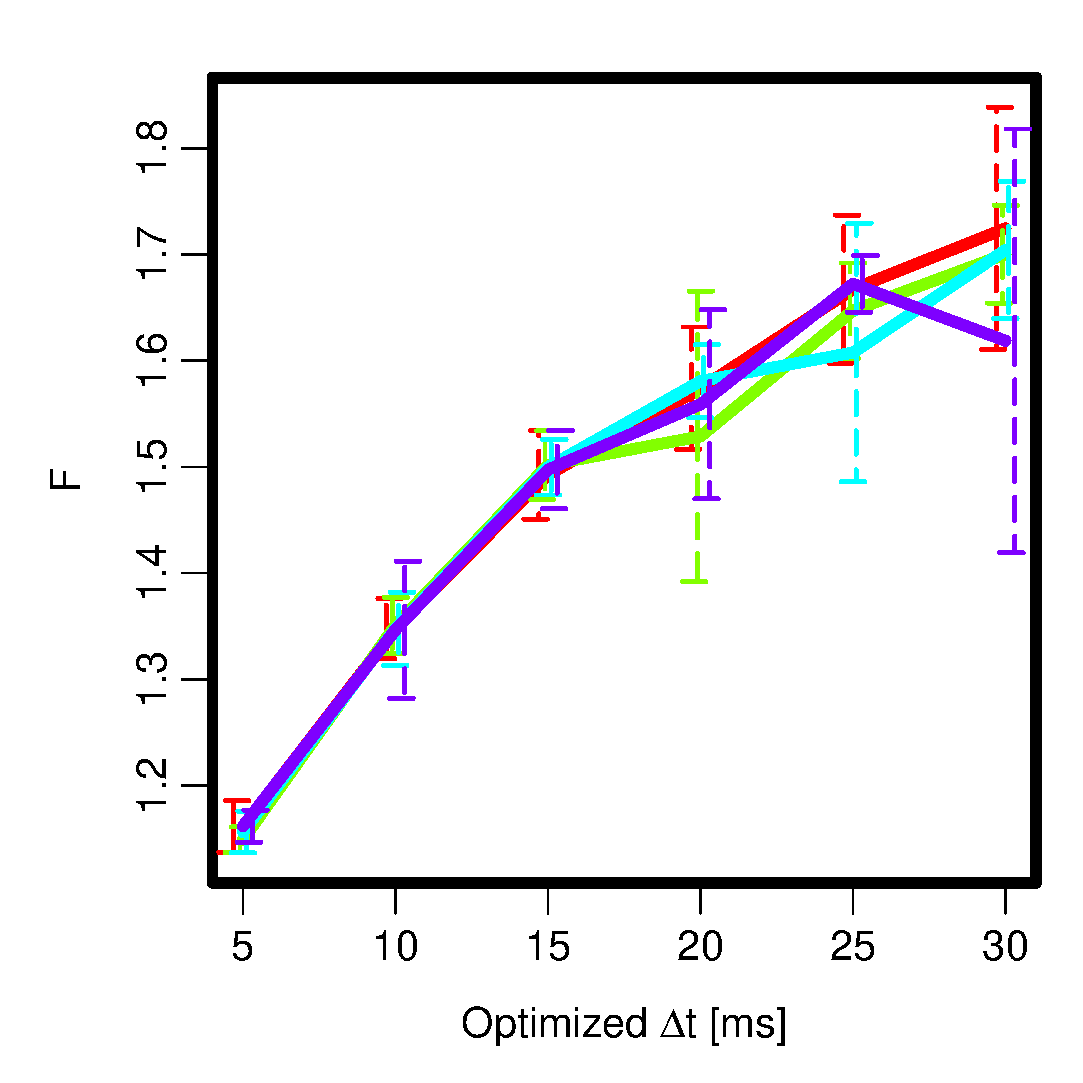
\includegraphics[width=0.8\columnwidth]{./Images_Result/ca_test_F.eps}
         \caption{F}
         \label{ca_F}
       \end{subfigure}
       \begin{subfigure}{0.5\columnwidth}
         \centering
         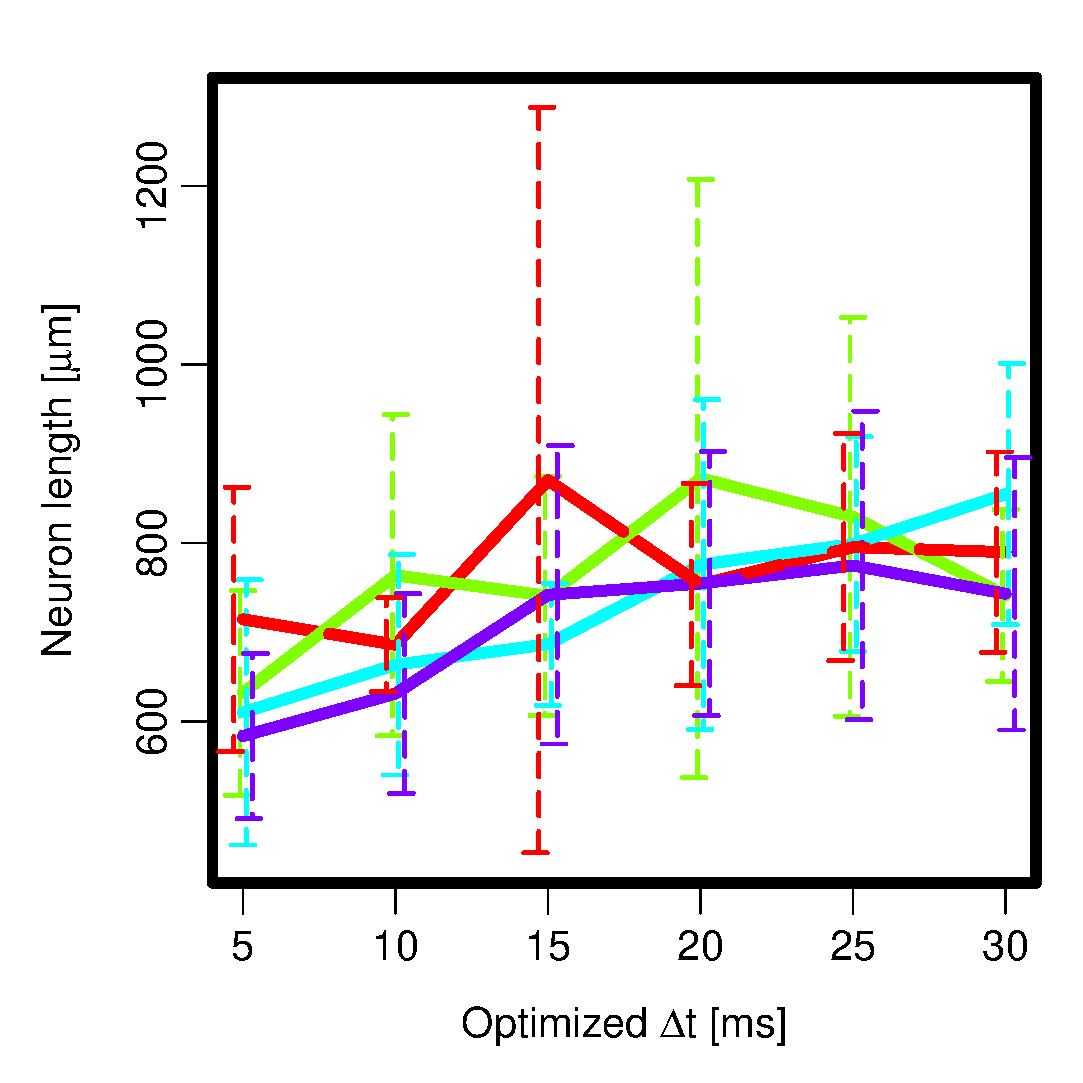
\includegraphics[width=0.8\columnwidth]{./Images_Result/ca_test_TREE_length.eps} 
         \caption{$BD9$5(B}
         \label{ca_TREE_length}
       \end{subfigure}

       \begin{subfigure}{0.5\columnwidth}
         \centering
         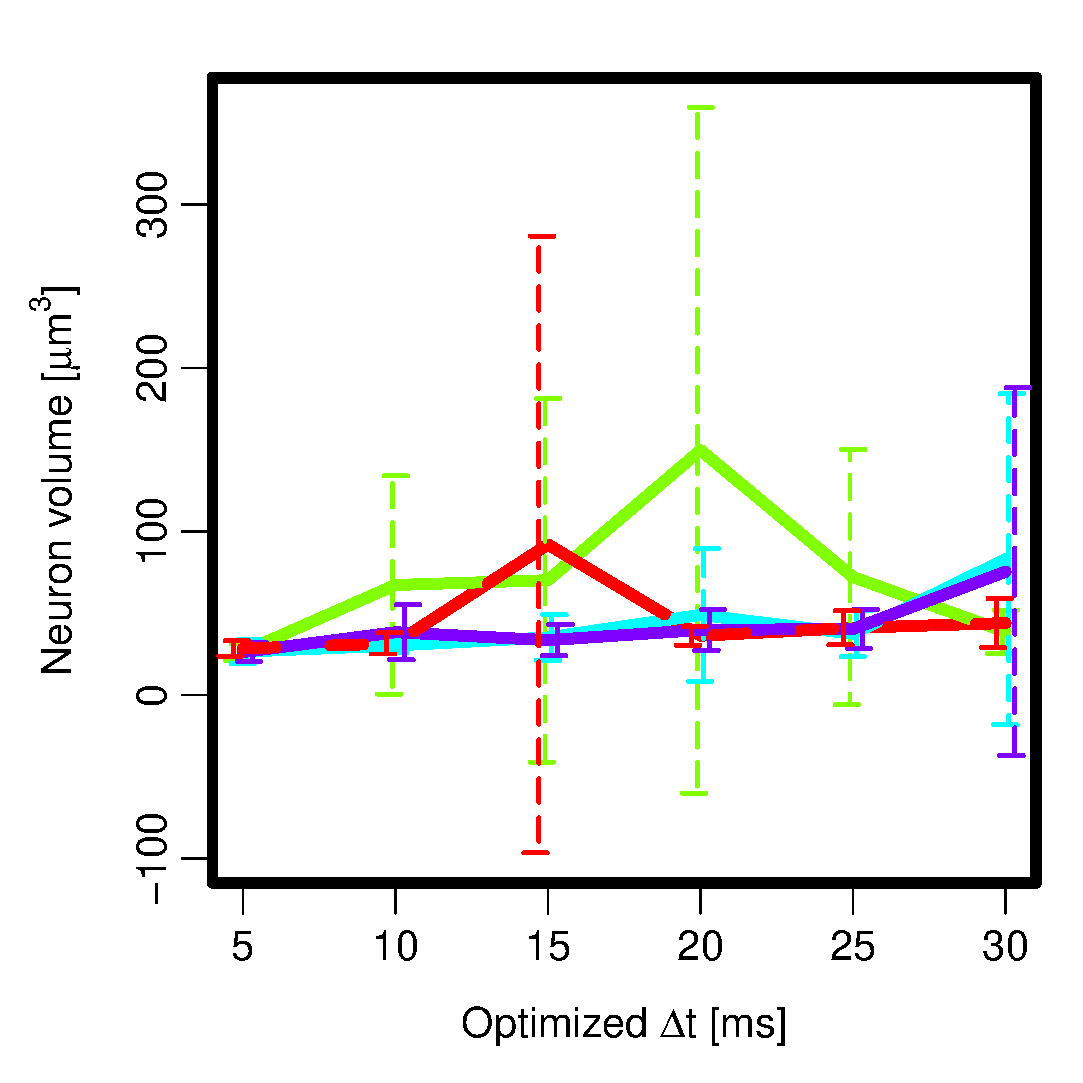
\includegraphics[width=0.8\columnwidth]{./Images_Result/ca_test_TREE_volume.eps}
         \caption{$BBN@Q(B}
         \label{ca_TREE_volume}
       \end{subfigure}
       \begin{subfigure}{0.5\columnwidth}
         \centering
         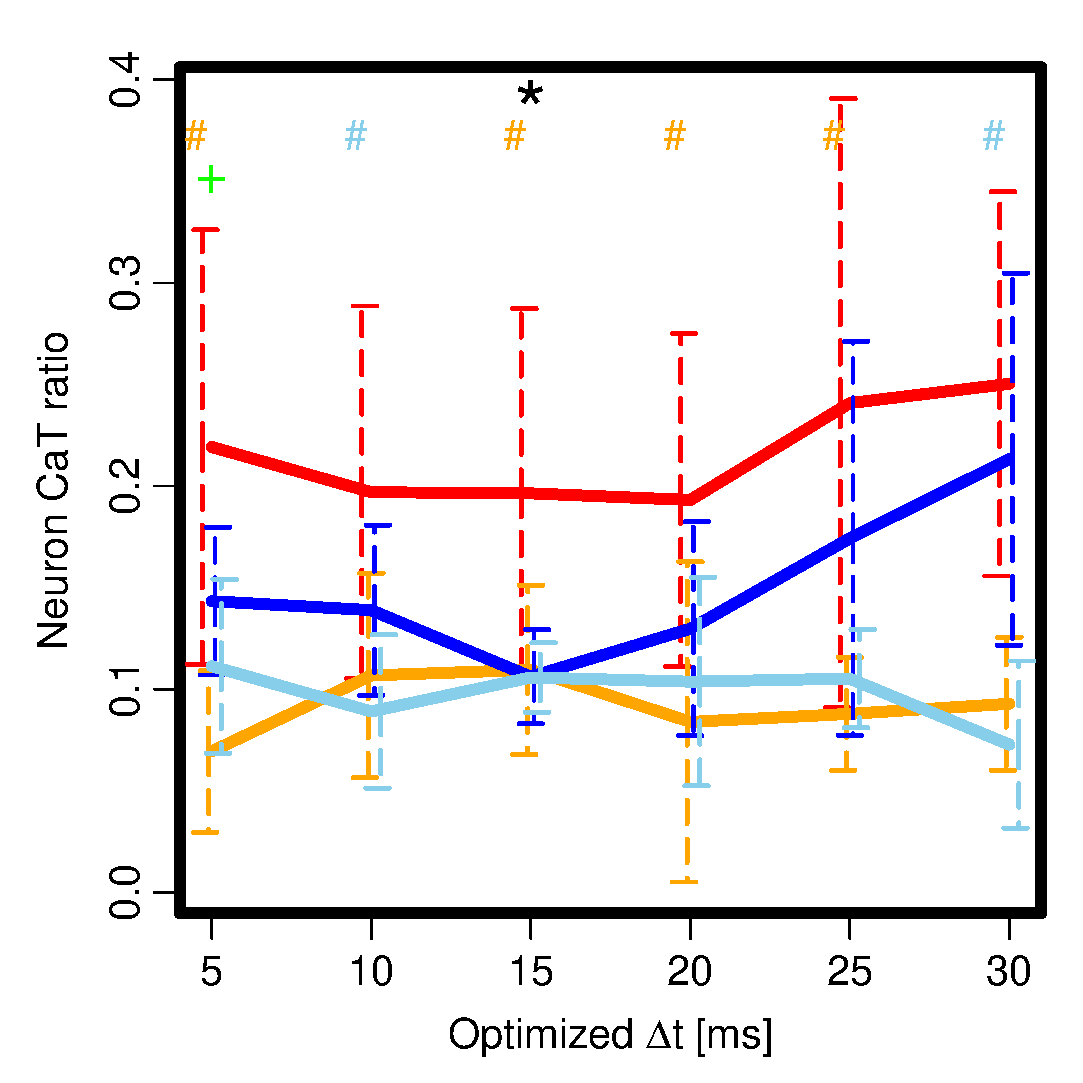
\includegraphics[width=0.8\columnwidth]{./Images_Result/ca_test_TREE_Ca_ratio.eps}
         \caption{CaT$B%3%s%@%/%?%s%94^M-N((B}
         \label{ca_TREE_Ca_ratio}
       \end{subfigure}
       
       \begin{subfigure}{0.5\columnwidth}
         \centering
         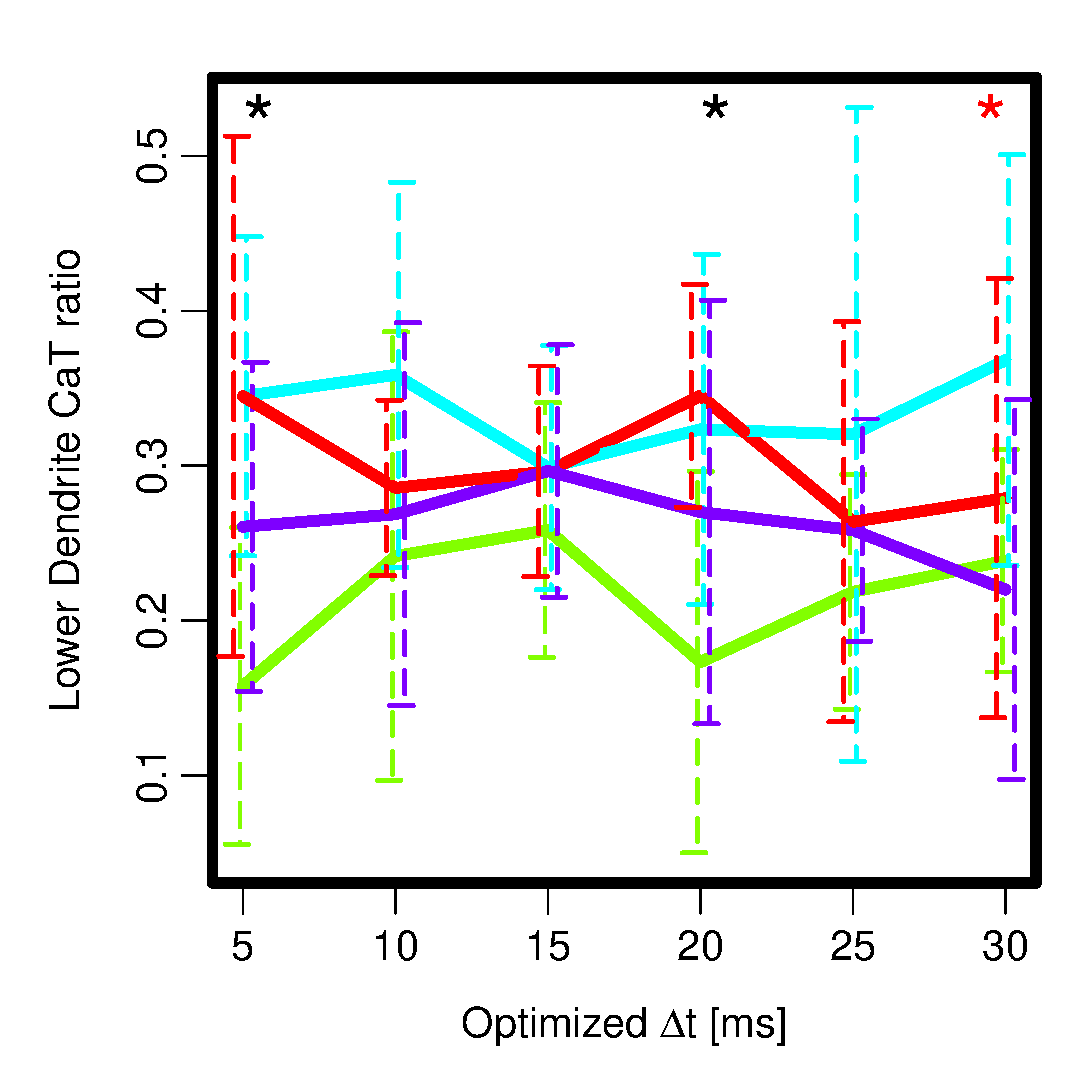
\includegraphics[width=0.8\columnwidth]{./Images_Result/ca_test_Lower_Ca_ratio.eps}
         \caption{Lower Dendrite$B$N(BCaT$B%3%s%@%/%?%s%94^M-N((B}
         \label{ca_lower_ratio}
       \end{subfigure}
       \begin{subfigure}{0.5\columnwidth}
         \centering
         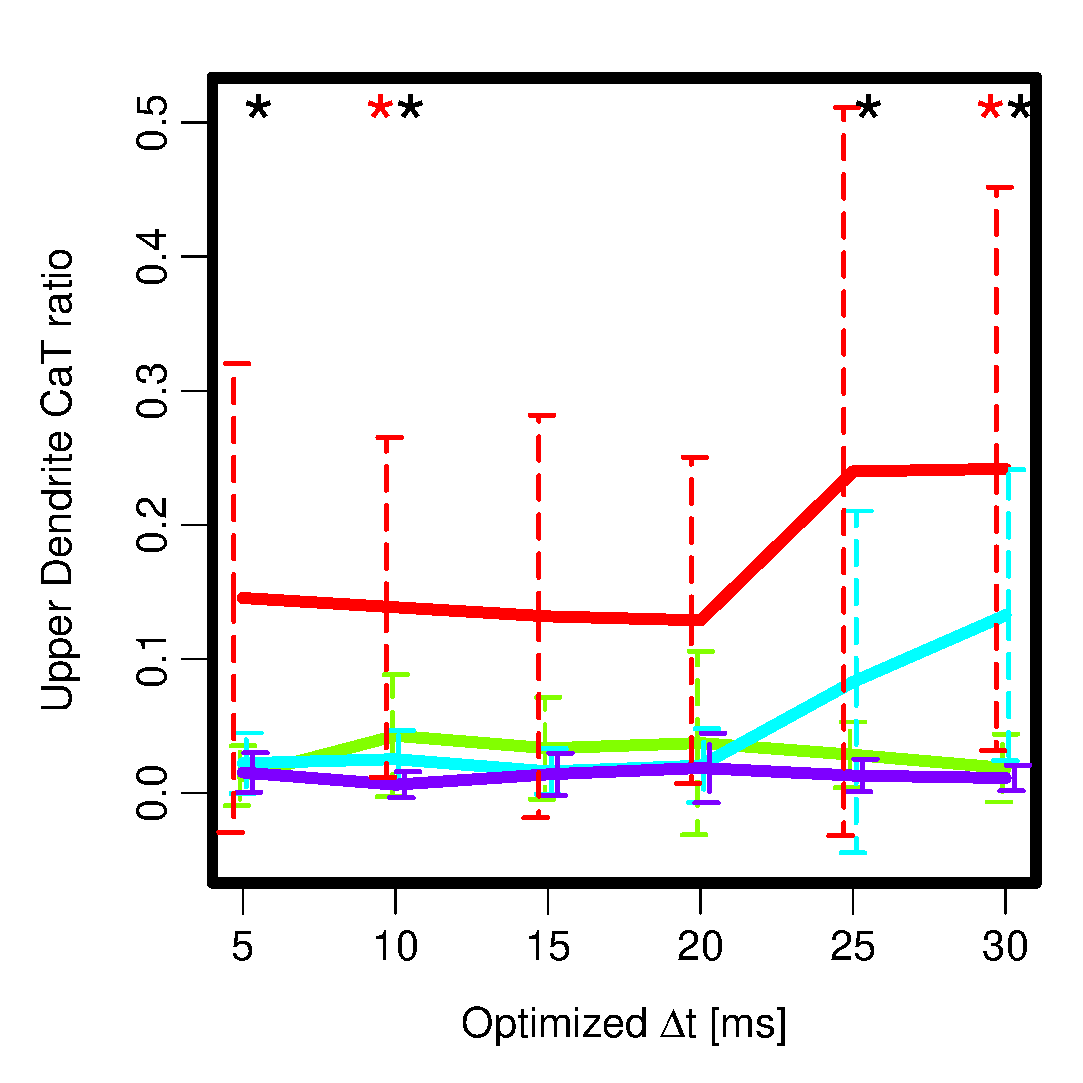
\includegraphics[width=0.8\columnwidth]{./Images_Result/ca_test_Upper_Ca_ratio.eps}
         \caption{Upper Dendrite$B$N(BCaT$B%3%s%@%/%?%s%94^M-N((B}
         \label{ca_upper_ratio}
       \end{subfigure}
       
       \vspace{-0.3cm}
       \begin{subfigure}{0.5\columnwidth}
         \centering
         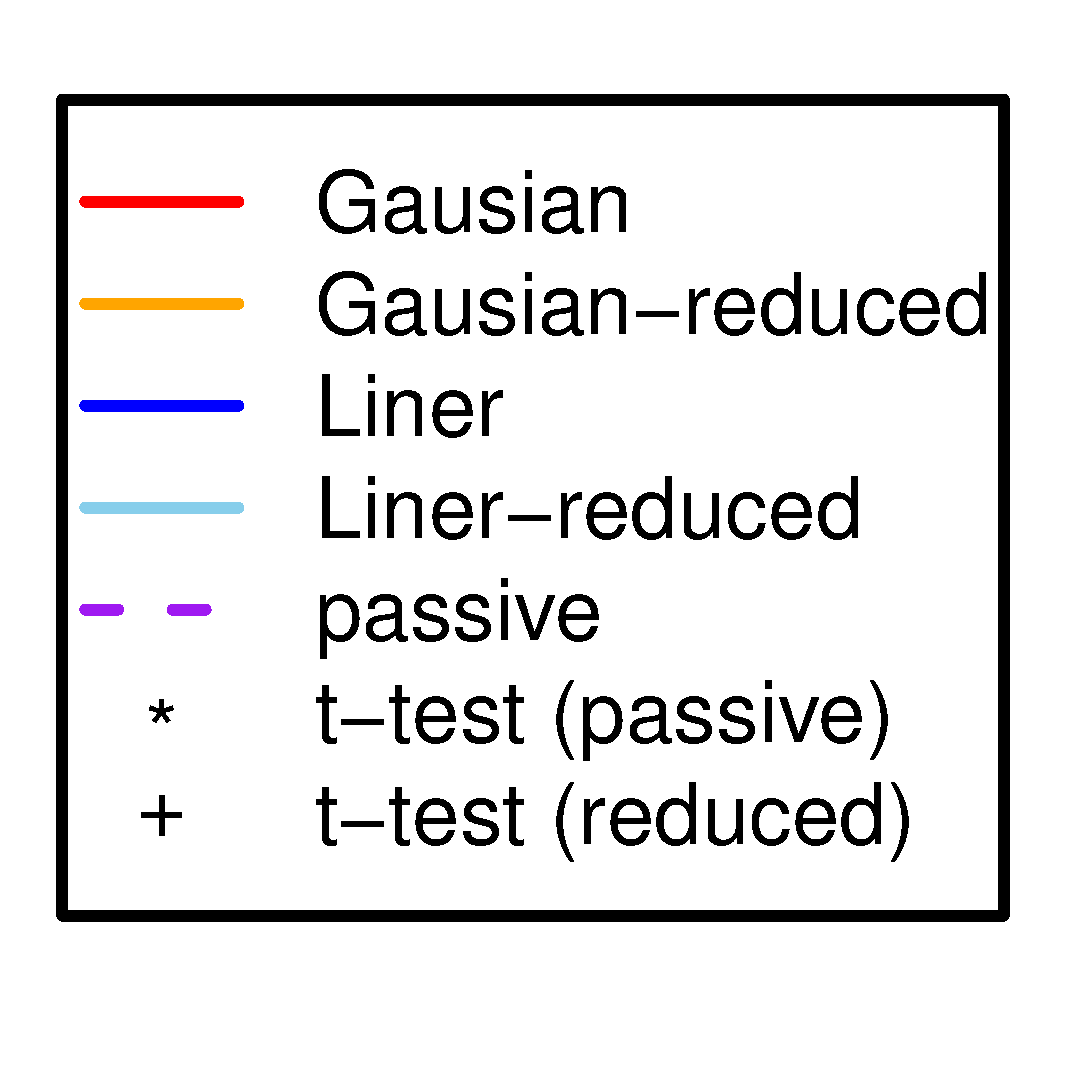
\includegraphics[width=0.6\columnwidth]{./Images_Result/ca_test_legend.eps} 
       \end{subfigure}
       \begin{subfigure}{0.5\columnwidth}
         \centering
         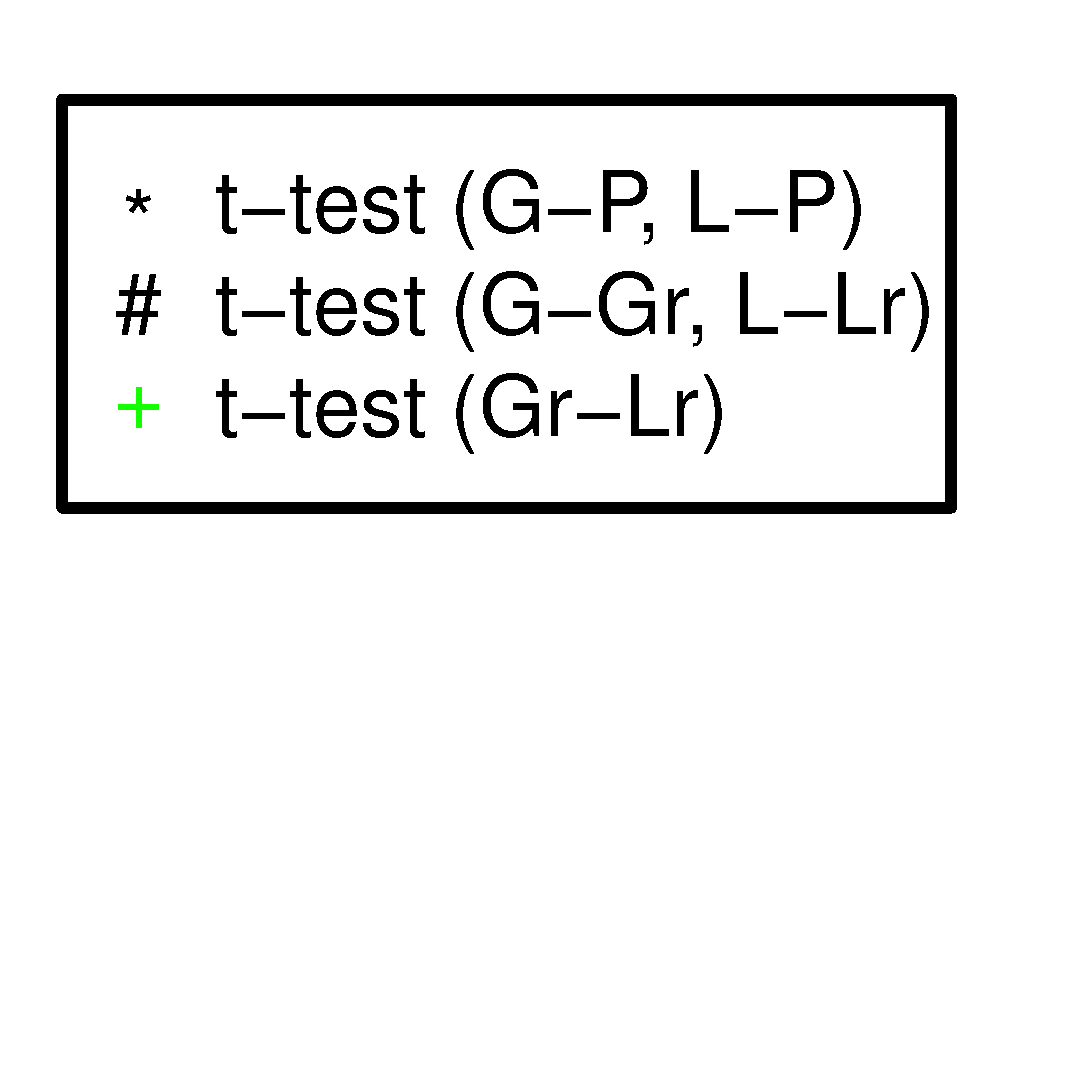
\includegraphics[width=0.6\columnwidth]{./Images_Result/test_legend.eps} 
       \end{subfigure}

       \vspace{-1.6cm}
       \caption{CaT$B%A%c%M%k$rF3F~$7$?:]$N7k2L(B} %$B%Z!<%8%l%$%"%&%H$,7hDj$7$F$+$iHyD4@0$9$k(B
       \label{ca_result}
     \end{figure}

     $B?^(B\ref{ca_F}$B$h$j(B, CaT$B%3%s%@%/%?%s%9$rF3F~$7$?$3$H$K$h$j(BPassive$B$N>l9g$h$j$b(B
     $F$$BCM$,A}2C$7$F$$$k$3$H$,$o$+$k(B. $B$^$?(BKa$B%3%s%@%/%?%s%9$N>l9g$H$O0c$C$F(B${\Delta}t$$B$,(B
     $BA}2C$9$k$[$IBg$-$J(B$F$$BCM$r$H$C$F$$$k(B.
     $B$3$l$O@h9T8&5f$G$b3NG'$5$l$F$$$k;v$G$"$k(B.\cite{torben2009systematic} \\
     $B?^(B\ref{Ca_morphos}$B$K(BCa$B%A%c%M%k$rF3F~$7$??@7P:YK&$N7ABVNc$r<($9(B. %$B%3%s%@%/%?%s%9$"$j$N>l9g$O$I$&$$$&7ABV$r$O$k$+!)(B
     \begin{figure}[H]
       \begin{subfigure}{0.5\columnwidth}
         \centering
         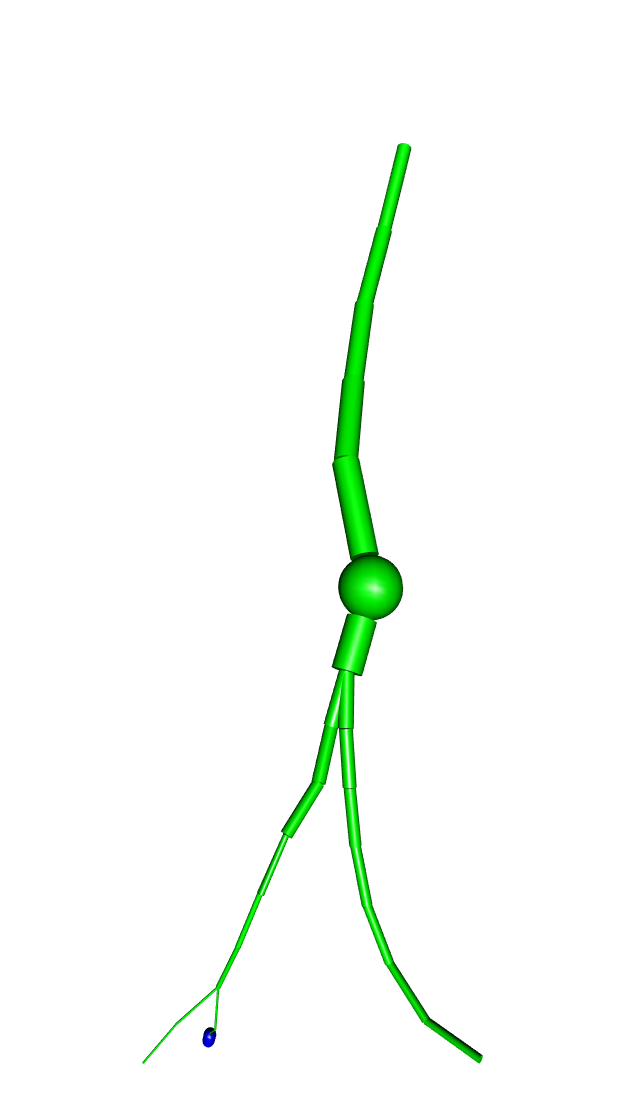
\includegraphics[width=0.5\columnwidth]{./Images_Result/alfa_sample.png} 
         \caption{$B@h9T8&5f<jK!(B}
      \label{Tsuishi_sampel}
       \end{subfigure}
       \begin{subfigure}{0.5\columnwidth}
         \centering
         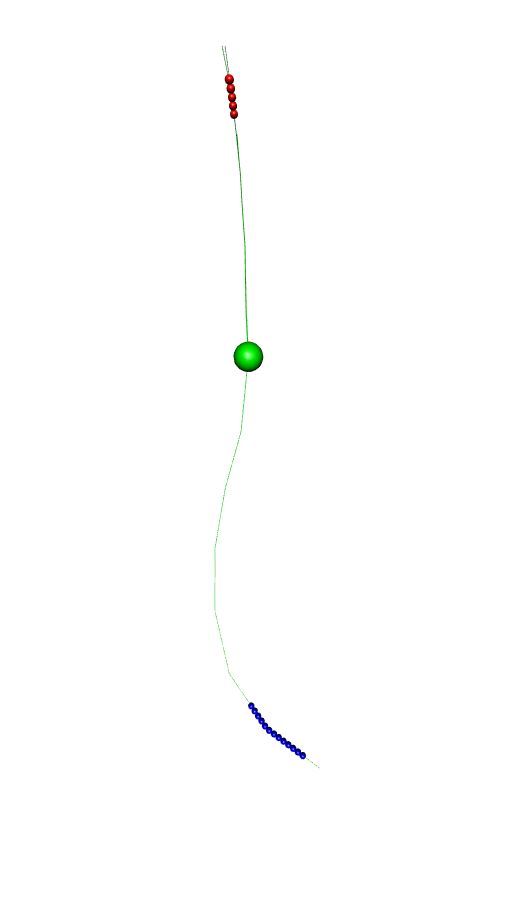
\includegraphics[width=0.3\columnwidth]{./Images_Result/rerative_sample.png}
         \caption{$BK\8&5f<jK!(B}
         \label{Rerative_sampel}
       \end{subfigure}
       \caption{CaT$B%3%s%@%/%?%s%9$rF3F~$7$??@7P:YK&$N7ABVNc(B}
       \label{Ca_morphos}
     \end{figure}

     $B?^(B\ref{ca_Ca_dist}$B$K(B${\Delta}t = 30$[ms]$B$H$7$F:n@.$7$??@7P:YK&$N(B
     $B%3%s%@%/%?%s%9J,I[$r<($9(B.
     $B?^(B\ref{ca_liner_dist}$B$H?^(B\ref{ca_liner_reduced_dist}$B$O@~7AJ,I[$rMQ$$(B,
     $B?^(B\ref{ca_gaus_dist}$B$H?^(B\ref{ca_gaus_reduced_dist}$B$O%,%&%9J,I[$rMQ$$$F$$$k(B.
     $B?^(B\ref{ca_line_reduced_dist}$B$H?^(B\ref{ca_gaus_reduced_dist}$B$O8DBNI>2A$K(B
     $B%3%s%@%/%?%s%9$N9MN8$rF~$l$?>l9g(B(reduced)$B$G$"$k(B. 
          %
          %$B!!?^$r:n$jD>$9(B
          %
     \begin{figure}[H]
       \hspace*{-4cm}
       \begin{subfigure}{0.68\columnwidth}
         \centering
         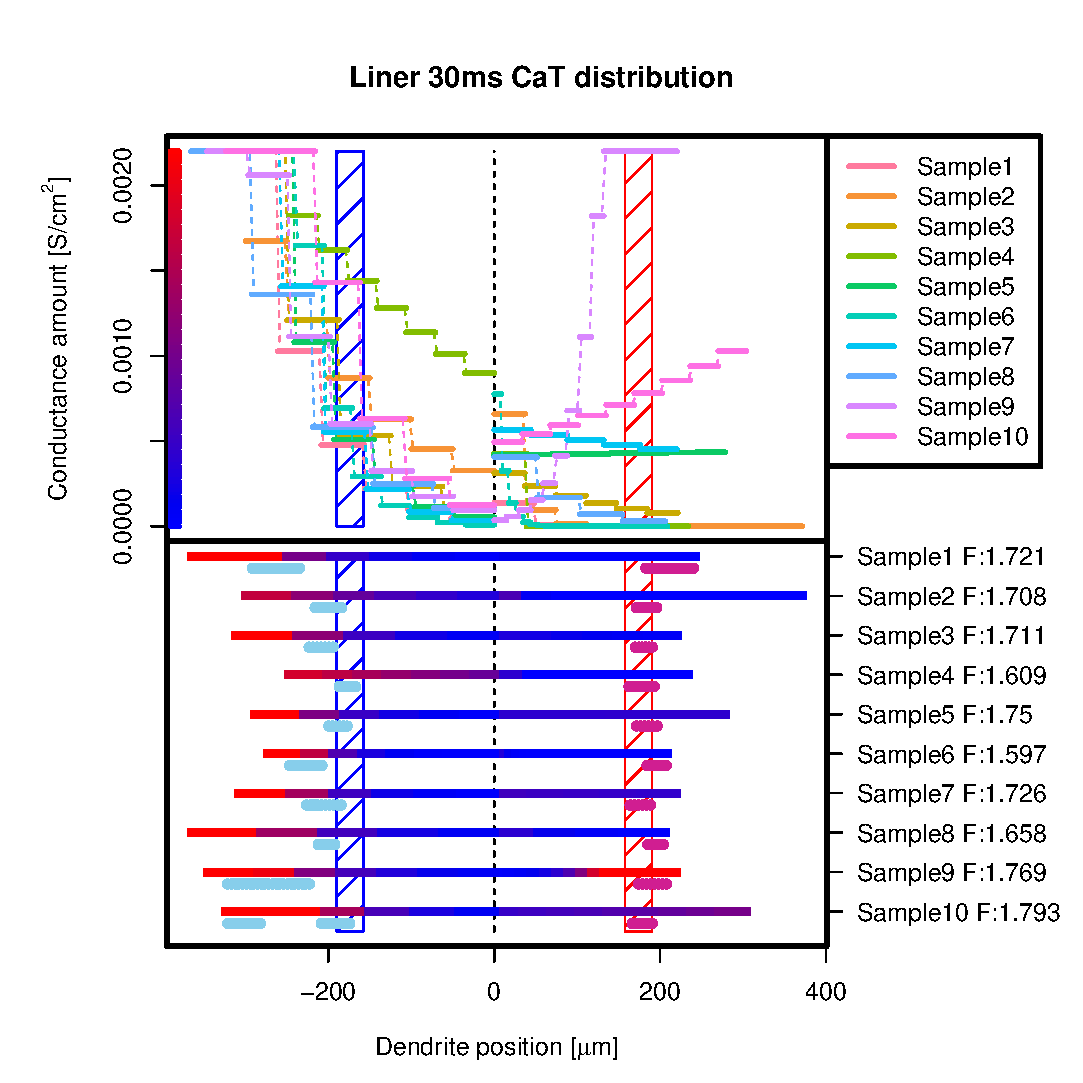
\includegraphics[width=\columnwidth]{./Images_Result/ca_Rerative_liner_75_0_Ca_distribution_dt30.eps}
         \caption{$B@~7AJ,I[(B}
         \label{ca_liner_dist}
       \end{subfigure}
       \begin{subfigure}{0.68\columnwidth}
         \centering
         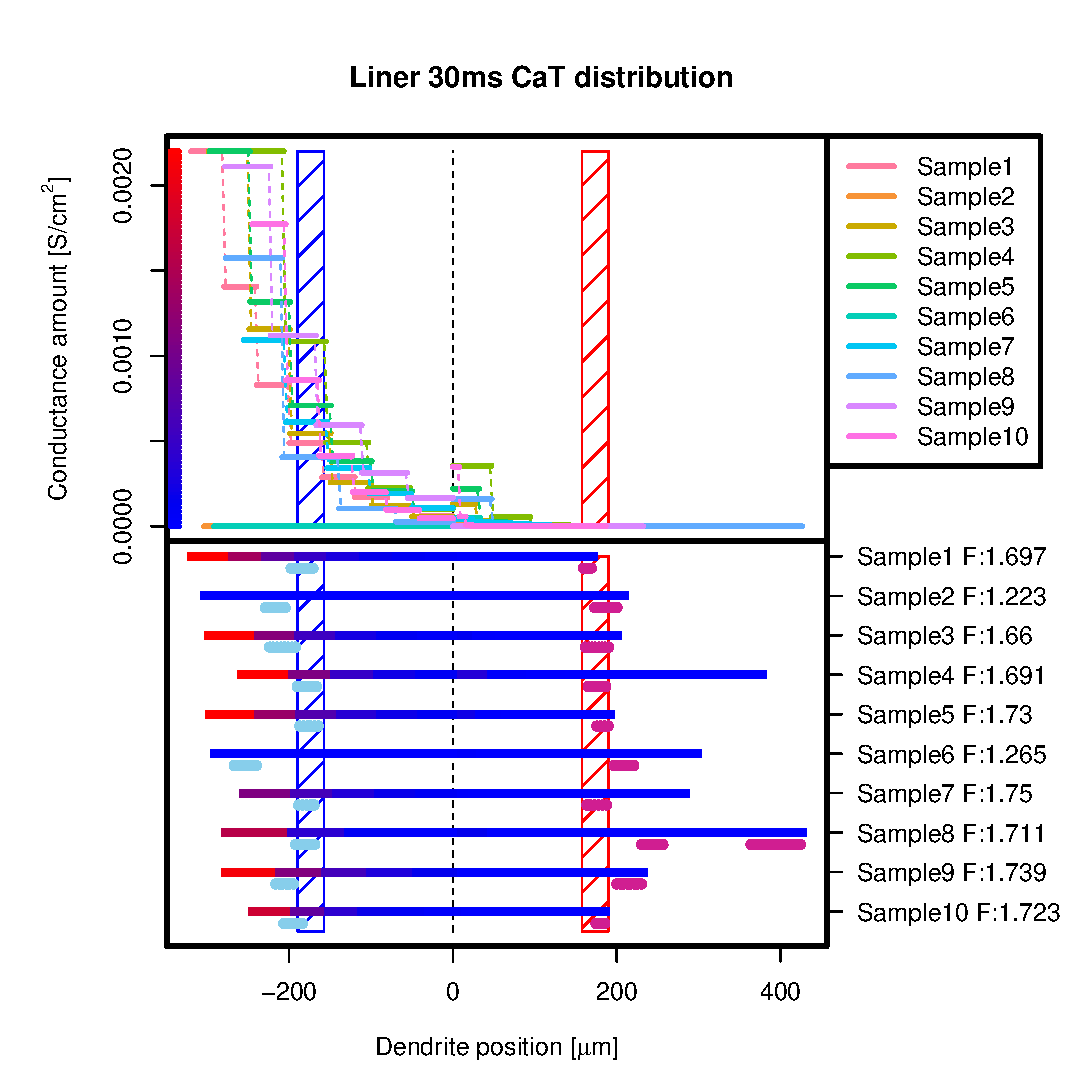
\includegraphics[width=\columnwidth]{./Images_Result/ca_Rerative_liner_75_5_Ca_distribution_dt30.eps}
         \caption{$B@~7AJ,I[(B(reduced)}
         \label{ca_liner_reduced_dist}
       \end{subfigure}

       \hspace*{-4cm}
       \begin{subfigure}{0.68\columnwidth}
         \centering
         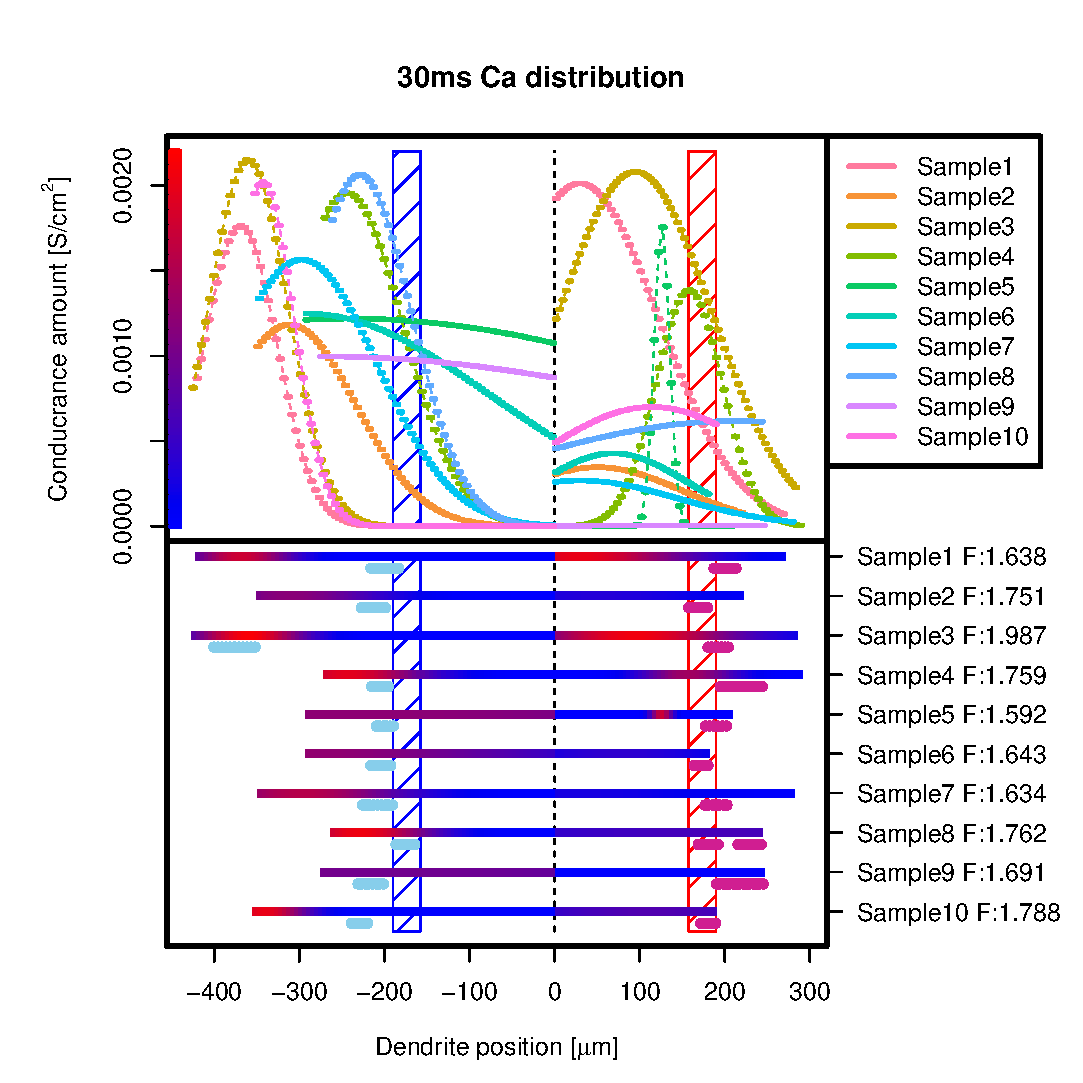
\includegraphics[width=\columnwidth]{./Images_Result/ca_Rerative_Gaus_75_0_Ca_distribution_dt30.eps}
         \caption{$B%,%&%9J,I[(B} %$B$3$N%,%&%9J,I[$N?^$O%7%J%W%F%#%C%/%>!<%s$r:n$jD>$7$?$[$&$,$$$$(B
         \label{ca_gaus_dist}
       \end{subfigure}
              \begin{subfigure}{0.68\columnwidth}
         \centering
         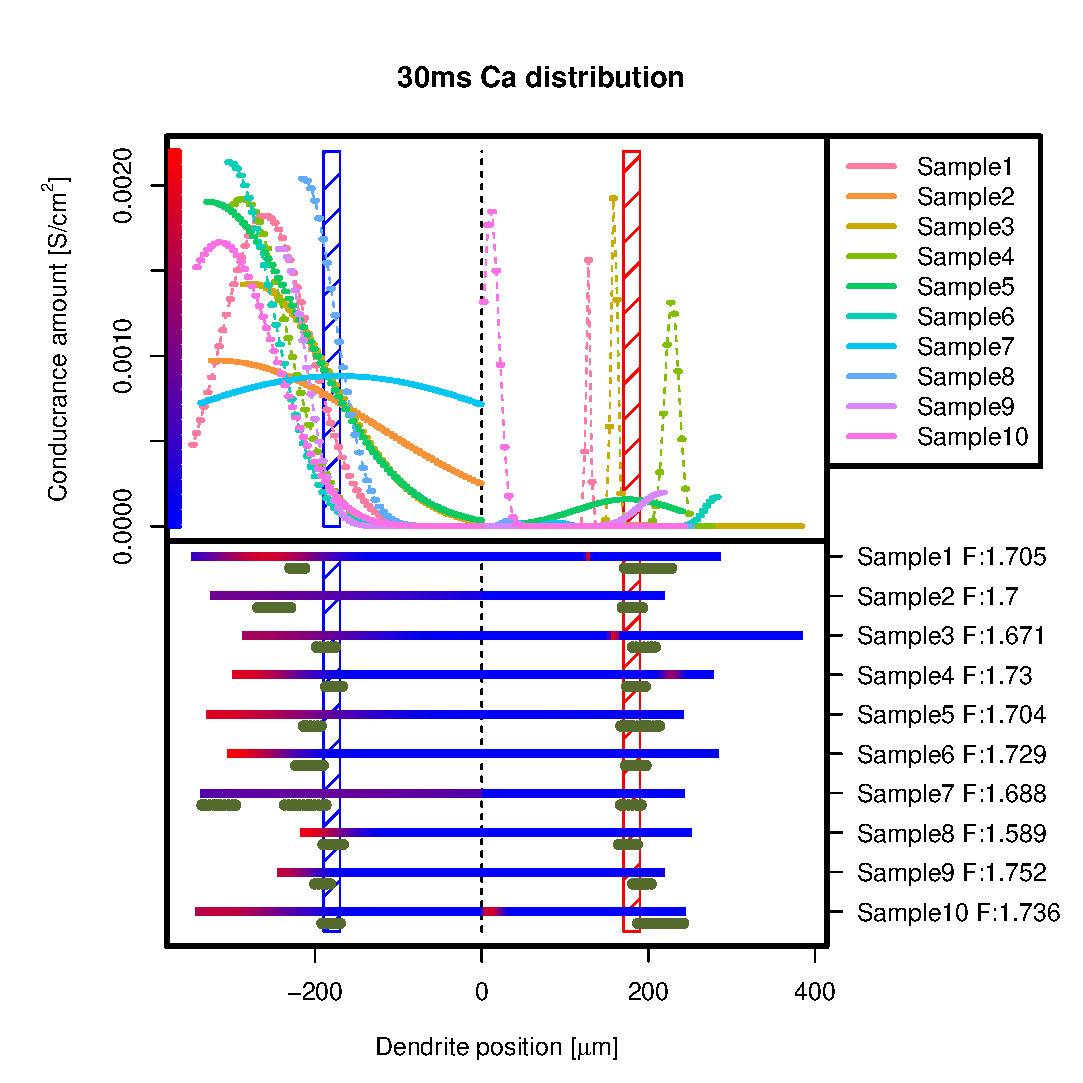
\includegraphics[width=\columnwidth]{./Images_Result/ca_Rerative_Gaus_75_5_Ca_distribution_dt30.eps}
         \caption{$B%,%&%9J,I[(B(reduced)} %$B$3$N%,%&%9J,I[$N?^$O%7%J%W%F%#%C%/%>!<%s$r:n$jD>$7$?$[$&$,$$$$(B
         \label{ca_gaus_reduced_dist}
       \end{subfigure}
       
       \begin{subfigure}{\columnwidth}
         \centering
         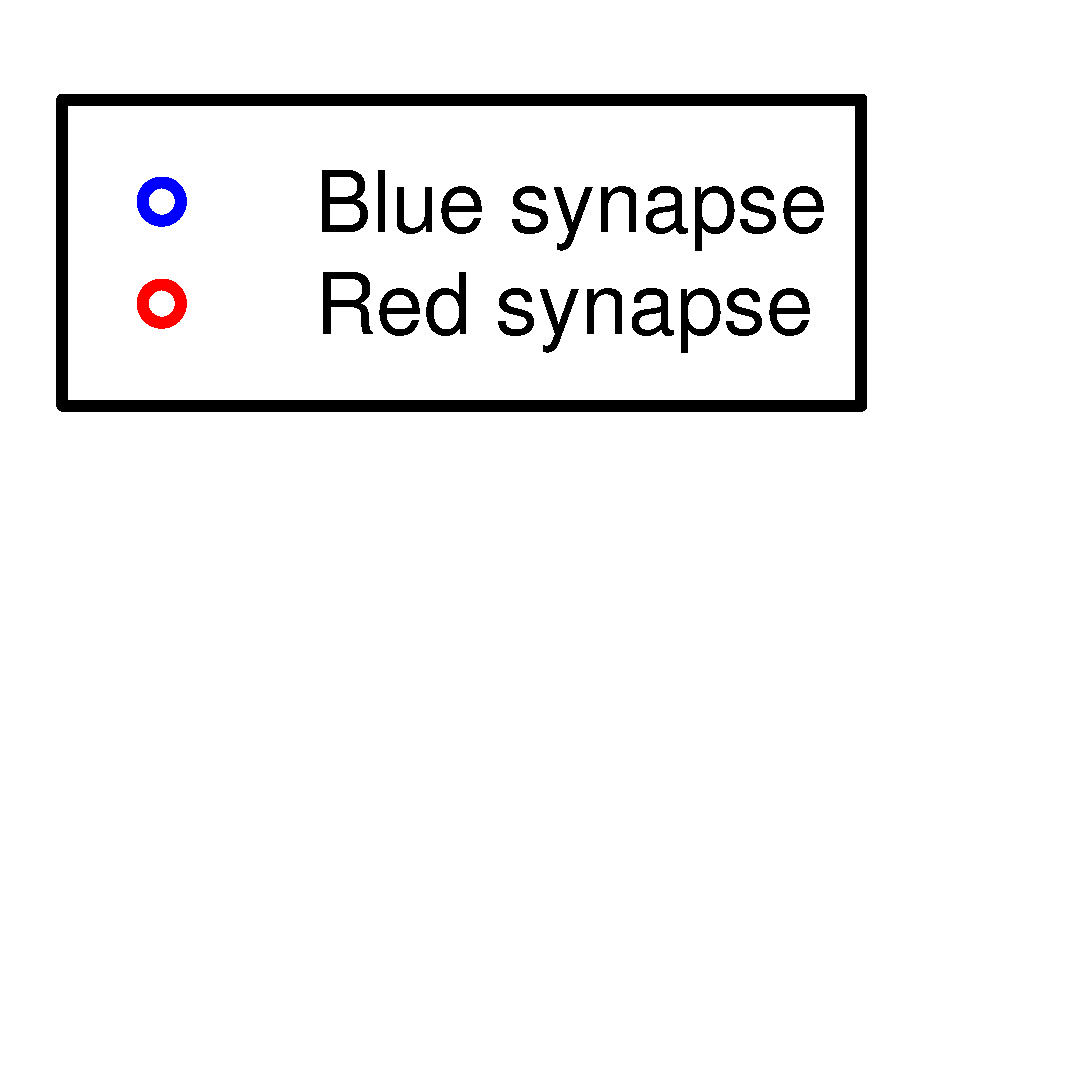
\includegraphics[width=0.35\columnwidth]{./Images_Result/Synapse_legend.eps} 
       \end{subfigure}
       
       \vspace{-3cm}
       \caption{${\Delta}t = 30$[ms], $B$G$N(BCaT$B%3%s%@%/%?%s%9J,I[(B}
       \label{ca_Ca_dist}
     \end{figure}

     $B?^(B\ref{ca_Ca_dist}$B$h$j(B, $B%3%s%@%/%?%s%9J,I[MM<0$K8B$i$:(BCaT$B%3%s%@%/%?%s%9$O(BLower Dendrite$B$N(B%$B<y>uFM5/$N8F$SJ}$r$I$&$9$k$+(B
     $B@hC<$KB?$/J,I[$7$F$$$k$3$H$,$o$+$k(B. $B8DBNI>2A$K$F%3%s%@%/%?%s%9NL$rI>2A$7$J$$>l9g$O(BUpper
     Dendrite$B$G$b(BCaT$B%3%s%@%/%?%s%9$NJ,I[$,8+$i$l$k$,(B, $BI>2A$K%3%s%@%/%?%s%9$N9MN8$rF3F~$9$k$H(B
     $B$[$H$s$I8+$i$l$J$/$J$C$?(B.
     
 \section{Ka$B%A%c%M%k(B, CaT$B%A%c%M%k$rMQ$$$?>l9g$N7k2L(B}

% $B:G8e$K$=$l$>$l$NJ,I[%Q%?!<%s!"%3%s%@%/%?%s%99MN8$NAH$G!"(B4$B%Q%?!<%s$N%3%s%@%/%?%s%9$K$h$k7k2L$r0l$D$N%0%i%U$K$^$H$a$k(B
